\documentclass[12pt]{article}

\usepackage{booktabs}% http://ctan.org/pkg/booktabs
\usepackage[utf8]{inputenc}
\usepackage{changepage}
\usepackage{pgfplots}
\usepackage{amssymb}
\usepackage{xcolor}
\usepackage{hyperref}
\usepackage{listings}
\usepackage[T1]{fontenc}
\usepackage[utf8]{inputenc}
\usepackage{adjustbox}
\usepackage{amsmath}
\usepackage{mathtools}
\usepackage{biblatex}
\usepackage{float}
\lstset{
  language=Python,
  numbers=left,
  numberstyle=\tiny,
  stepnumber=1,
  numbersep=5pt,
  tabsize=4,
  basicstyle=\ttfamily,
  columns=fullflexible,
  keepspaces,
}
\hypersetup{
    colorlinks,
    citecolor=black,
    filecolor=black,
    linkcolor=black,
    urlcolor=black
}

% Set page size and margins
% Replace `letterpaper' with `a4paper' for UK/EU standard size
\usepackage[letterpaper,top=2cm,bottom=2cm,left=3cm,right=3cm,marginparwidth=1.75cm]{geometry}

% Useful packages
\usepackage{amsmath}
\usepackage{mathtools}
\usepackage{graphicx}
\newenvironment{para}{\begin{adjustwidth}{13mm}{}}{\end{adjustwidth}}

\newcommand\tab[1][1cm]{\hspace*{#1}}

\newcommand{\tabitem}{\llap{\textbullet}}
\newcommand{\Hsquare}{%
\text{\fboxsep=-.2pt\fbox{\rule{0pt}{1ex}\rule{1ex}{0pt}}}%
}

\newtheorem{Definizione}{Definizione}[subsection]
\newtheorem{Lemma}{Lemma}[subsection]
\newtheorem{Teorema/Definizione}{Teorema/Definizione}[subsection]
\newtheorem{Corollario}{Corollario}[subsection]
\newtheorem{Teorema}{Teorema}[subsection]
\newtheorem{Proposizione}{Proposizione}[subsection]
\newtheorem{Notazione}{Notazione}[subsection]
\newtheorem{Commento}{Commento}[subsection]
\newtheorem{Dimostrazione}{Dimostrazione}[subsection]
\newtheorem{Osservazione}{Osservazione}[subsection]
\newtheorem{Nota}{Nota}[subsection]

\title{RSO: Sistemi Operativi}
\author{spitfire}
\date{A.A. 2024-2025}
\begin{document}
\begin{figure}
    \centering
    
\includegraphics[width=0.35\textwidth]{Images/Logo scienze bicocca.png}
\end{figure}

\vspace{10cm}
\date{A.A. 2024-2025}


\maketitle

\newpage

\tableofcontents
\newpage

\section{Struttura e servizi}
Cosa sappiamo sui sistemi operativi? Sappiamo che, per esempio, i principali sono
\textbf{linux, Windows e MacOS}; che il sistema operativo è il 
\textbf{primo programma che viene eseguito dopo il boot}. Di solito un sistema operativo
fornisce un \textbf{ambiente desktop a finestre e ci permette di installare nuove applicazioni}.
Ci permette inoltre di eseguire tante applicazioni \textbf{contemporaneamente}, anche più dei \textbf{core dei processori}.
Inoltre, esso \textbf{mantiene e organizza i nostri dati sotto forma di file e cartelle}.
Quindi, cos'è un \textbf{sistema operativo}? Esso è:
\begin{itemize}
    \item Un insieme di \textbf{programmi} (Software)
    \item Che gestiscono \textbf{gli elementi fisici di un computer} (Hardware)
\end{itemize}
E a \textbf{cosa serve un sistema operativo}?
\begin{itemize}
    \item Fornire una \textbf{piattaforma di sviluppo per le applicazioni}, che permette loro di \textbf{condividere e astrarre} le risorse HW.
    \item Agisce da \textbf{intermediario} tra utenti e computer, permettendo agli utenti di \textbf{controllare l'esecuzione dei programmi applicativi} e l'assegnazione delle risorse HW ad essi
    \item \textbf{Protegge le risorse degli utenti} (e dei loro programmi) dagli altri utenti (e dai loro programmi) e da eventuali \textbf{attori esterni}
\end{itemize}
Un sistema operativo è quindi in primo luogo una \textbf{piattaforma di sviluppo}, ossia un insieme di funzionalità software che i programmi applicativi possono usare.
Tali funzionalità permettono ai programmi di poter usare in maniere conveniente le risorse hardware di condividerle:
\begin{itemize}
    \item Da un lato il sistema operativo \textbf{astrae} le risorse hardware, presentando agli sviluppatori di programmi applicativi una visione delle risorse hardware più facile da usare e più potente rispetto alle risorse hardware "native".
    \item Dall'altro, il sistema operativo \textbf{condivide} le risorse hardware tra molti programmi contemporaneamente in esecuzione, suddividendole tra i programmi in maniera equa ed efficiente e controllando che questi le usino correttamente.
\end{itemize}
\subsection{Componenti di un sistema di elaborazione}
Le componenti di un sistemi di elaborazione sono:
\begin{itemize}
    \item \textbf{Utenti}: Persone, macchine, altri computer, ecc...
    \item \textbf{Programmi applicativi}: Risolvono i problemi di calcolo degli utenti
    \item \textbf{Sistema operativo}: Coordina e controlla l'uso delle risorse hardware
    \item \textbf{Hardware}: Risorse di calcolo (CPU, periferiche, memoria di massa, ...)
\end{itemize}
\begin{center}
    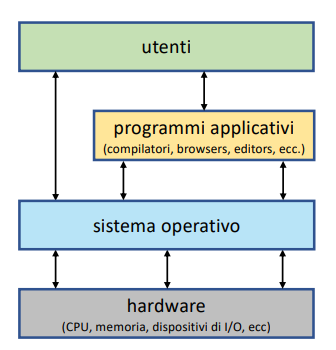
\includegraphics[width = 0.50\textwidth]{Images/1.PNG}
\end{center}
\subsection{Requisiti per i sistemi operativi}
Oggigiorno i computer sono ovunque: vi sono molteplici tipologie di computer utilizzati in scenari
applicativi molto diversi. In quasi tutti i tipi di computer si tende ad installare un sistema operativo allo scopo
di gestire l'hardware e semplificare la programmazione. Ma ogni scenario applicativo in cui viene usato un computer
richiede che il sistema operativo che vi viene installato abbia caratteristiche ben determinate. Che cosa si richiede quindi
ad un sistema operativo per supportare uno determinato scenario applicativo?
Vediamo qualche scenario:
\begin{itemize}
    \item \textbf{Server e Mainframe}: massimizzare le performance, rendere equa la condivisione delle risorse tra molti utenti
    \item \textbf{Laptop, PC e tablet}: massimizzare la facilità d'uso e la produttività della singola persona che lo usa
    \item \textbf{Dispositivi mobili}: Ottimizzare i consumi energetici e la connettività
    \item \textbf{Sistemi embedded}: funzionare senza, o con minimo, intervento umano e reagire in tempo reale agli stimoli esterni (interrupt)
\end{itemize}
\subsection{La maledizione della generalità}
Nella storia (ed anche oggi) alcuni sistemi operativi sono stati utilizzati per scenari applicativi diversi.
Ad esempio, Linux è usato oggi nei server, nei computer desktop e nei dispositivi mobili (come parte di Android).
La \textbf{maledizione della generalità} afferma che, se un sistema operativo deve supportare un insieme di scenari applicativi troppo ampio,
non sarà in grado di supportarne nessuno particolarmente bene. Esempio di questo si è visto con \textbf{OS/360}, il primo sistema operativo che doveva supportare
una famiglia di computer diversi (la linea 360 IBM).
\subsection{Struttura dei sistemi operativi}
Non c'è una definizione universalmente accettata di quali programmi fanno pare di un sistema operativo. In generale però un sistema operativo almeno comprende:
\begin{itemize}
    \item \textbf{Kernel}: Il "programma sempre presente" che si "impadronisce" dell'HW, lo gestisce, ed offre ai programmi i servizi per poterlo usare in maniera condivisa ed astratta
    \item \textbf{Middleware}: servizi di alto livello che astraggono ulteriormente i servizi del kernel e semplificano la programmazione di applicazioni (API, framework per grafica e per suono,...)
    \item \textbf{Programmi di sistema}: Non sempre in esecuzione, offrono ulteriori funzionalità di supporto e di interazione utente con il sistema (gestione di processi e jobs, UI, ...)
\end{itemize}
Alcuni sistemi operativi forniscono "out-of-the-box" anche dei \textbf{programmi applicativi} (editor, fogli di calcolo,...) ma non li considereremo come parti del sistema operativo.
Data questa lista di componenti, possiamo rivisitare le \textbf{componenti di un sistema di elaborazione}:
\begin{center}
    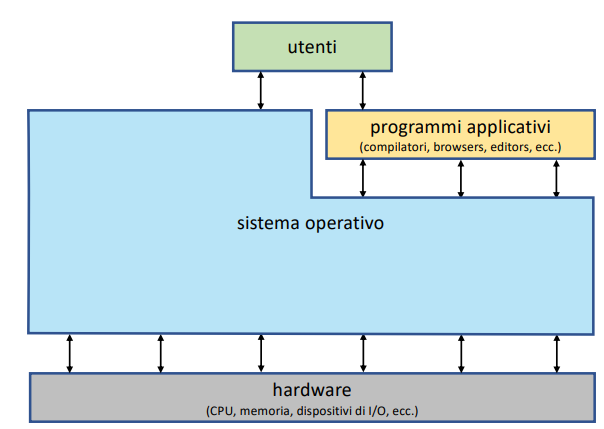
\includegraphics[width = 0.55\textwidth]{Images/2.PNG}
\end{center}
Che visti in dettaglio diventano:
\begin{center}
    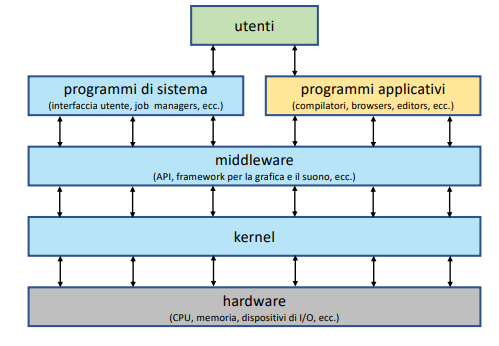
\includegraphics[width = 0.63\textwidth]{Images/3.PNG}
\end{center}
\subsection{Servizi offerti da un sistema operativo}
I principali servizi che un sistema operativo offre sono:
\begin{itemize}
    \item \textbf{Controllo processi}: questi servizi permettono di caricare in memoria un programma, eseguirlo, identificare la sua terminazione e registrarne la condizione di terminazione (normale o erronea)
    \item \textbf{Gestione dei file}: questi servizi permettono di leggere, scrivere e manipolare files e directories
    \item \textbf{Gestione dispositivi}: questi servizi permettono ai programmi di effettuare operazioni di input/output, ad esempio leggere da/scrivere su un terminale
    \item \textbf{Comunicazione interprocesso}: i programmi in esecuzione possono collaborare tra di loro scambiandosi informazioni: questi servizi permettono ai programmi in esecuzione di comunicare
    \item \textbf{Protezione e sicurezza}: permette ai proprietari delle informazioni in un sistema multiutente o in rete di controllarne l'uso da parte di altri utenti e di difendere il sistema dagli accessi illegali
    \item \textbf{Allocazione delle risorse}: alloca le risorse hardware (CPU, memoria, dispositivi di I/O) ai programmi in esecuzione in maniera equa ed efficiente
    \item \textbf{Rilevamento errori}: gli errori possono avvenire nell'hardware o nel software  (es. divisione per 0); quando avvengono il sistema operativo deve intraprendere opportune azioni (recupero, terminazione del programma o segnalazione della condizione di errore al programma)
    \item \textbf{Logging}: mantiene traccia di quali programmi usano quali risorse, allo scopo di contabilizzarle
\end{itemize}
\subsection{Chiamate di sistema e Application Programming Interfaces}
\begin{center}
    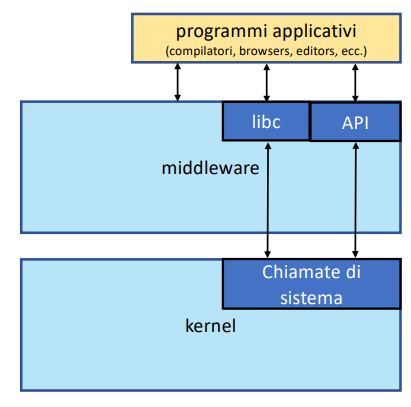
\includegraphics[width = 0.50\textwidth]{Images/4.PNG}
\end{center}
Il kernel offre i propri servizi ai programmi come \textbf{chiamate di sistema} (syscalls), ossia funzioni invocabili in un determinato linguaggio di programmazione (C, C++, ...).
I programmi però non utilizzano direttamente le chiamate di sistema, ma delle librerie di middleware dette \textbf{Application Programming Interface} (API) implementate invocando le chiamate di sistema.
Spesso le API sono fortemente legate con le librerie standard del linguaggio di implementazione (es. libc se le API sono implementate in C) al punto che anche queste diventano parte implicita dell'API.
Bisogna ricordare che:
\begin{itemize}
    \item Le API sono \textbf{esposte dal middleware}, mentre le chiamate di sistema \textbf{dal kernel}
    \item Le API usano le chiamate di sistema nella loro implementazione
    \item Le API sono standardizzate (es. POSIX, Win32), le chiamate di sistema no, quindi ogni kernel ha chiamate di sistema differenti
    \item Le API sono stabili, le chiamate di sistema possono variare al variare della versione del sistema operativo
    \item Le API offrono funzionalità più ad alto livello e più semplici da usare, le chiamate di sistema offrono funzionalità più elementari e più complesse da usare
\end{itemize}
\begin{center}
    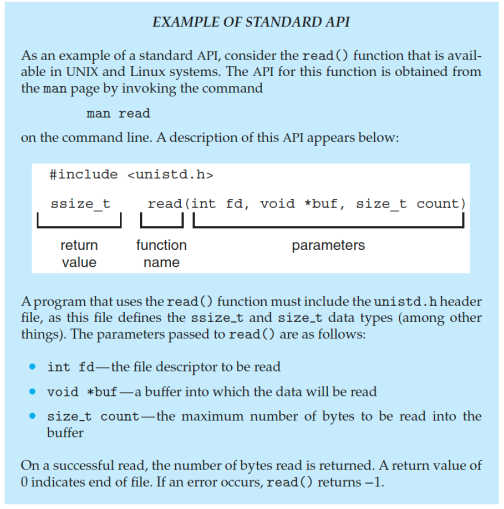
\includegraphics[width = 0.75\textwidth]{Images/5.PNG}
\end{center}
\subsection{Programmi di sistema}
La maggior parte degli utenti utilizza servizi del sistema operativo attraverso i programmi di sistema.
Questi permettono agli utenti di avere un ambiente più conveniente per l'esecuzione dei programmi, il loro sviluppo e la gestione delle risorse del sistema.
Vi sono diversi tipi di programmi di sistema:
\begin{itemize}
    \item \textbf{Interfacce utente (UI)}: permette agli utenti di interagire con il sistema stesso; può essere grafica (GUI) o a riga di comando (CLI); i sistemi mobili hanno un'interfaccia touch.
    \item \textbf{Gestione file}: creazione, modifica e cancellazione di file e directories
    \item \textbf{Modifica dei file}: editor di testo, programmi per la manipolazione del contenuto dei file (Emacs)
    \item \textbf{Visualizzazione e modifica informazioni di stato}: data, ora, memoria disponibile, processi, utenti, ... fino a informazioni complesse su prestazione, accessi al sistema e debug. Alcuni sistemi implementano un \textbf{registry}, ossia un database delle informazioni di configurazione
    \item \textbf{Caricamento ed esecuzione dei programmi}: loader assoluti e rilocabili, linker e debugger
    \item \textbf{Ambienti di supporto alla programmazione}: compilatori, assemblatori, debugger, interpreti per diversi linguaggi di programmazione
    \item \textbf{Comunicazione}: forniscono i meccanismi per creare connessione tra utenti, programmi e sistemi; permettono di inviare messaggi agli schermi di un altro utente, di navigare il web, di inviare messaggi di posta elettronica, di accedere remotamente ad un altro computer, di trasferire i file, ecc...
    \item \textbf{Servizi di background}: lanciati all'avvio, alcuni terminano, altri continuano l'esecuzione fino allo shutdown. Forniscono servizi quali verifica dello stato dei dischi, scheduling di jobs, logging, ...
\end{itemize}
\subsubsection{Intefaccia utente: l'interpete dei comandi}
\begin{center}
    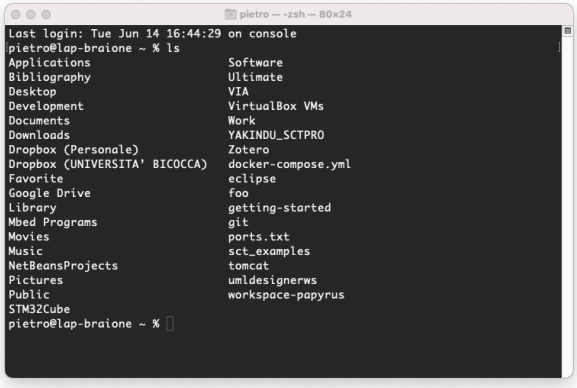
\includegraphics[width = 0.75\textwidth]{Images/6.PNG}
\end{center}
L'interprete dei comandi permette agli utenti di impartire in maniera testuale delle istruzioni al sistema operativo.
In molti sistemi operativi è possibile configurare quale interprete dei comandi usare, nel qual caso è detto \textbf{shell}.
Ci sono due modi per implementare un comando:
\begin{itemize}
    \item \textbf{Built-in}: l'interprete esegue direttamente il comando (tipico dell'interprete dei comandi di Windows)
    \item \textbf{Come programma di sistema}: l'interprete manda in esecuzione un programma (tipico delle shell Unix e Unix-Like)
\end{itemize}
Spesso l'interprete riconosce \textbf{un vero e proprio linguaggio di programmazione} (es. Bash).
\subsubsection{Interfaccia utente: le interfacce grafiche}
\begin{center}
    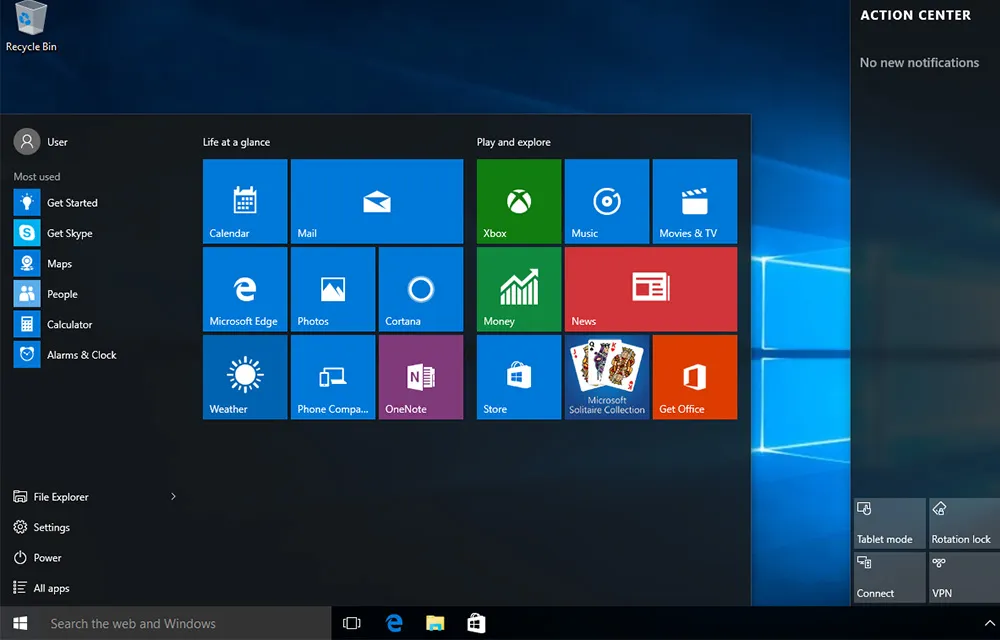
\includegraphics[width = 0.85\textwidth]{Images/7.png}
\end{center}
Le interfacce grafiche(GUI) sono di solito basate sulla metafora della scrivania, delle icone e delle cartelle (corrispondenti alle directory).
Nate dalla ricerca presso lo Xerox PARC lab negli anni 70, vennero popolarizzate dai computer Apple Macintosh negli anni 80. Su Linux le più popolari sono KDE e Gnome.
\newpage
\subsubsection{Intefaccia utente: Le interfacce touch-screen}
\begin{center}
    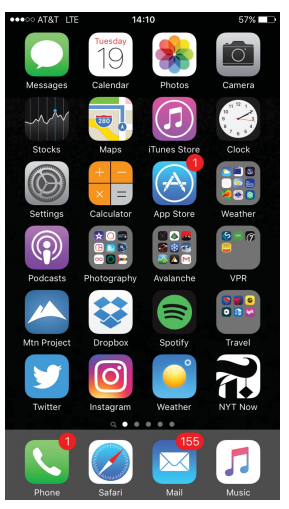
\includegraphics[width = 0.30\textwidth]{Images/8.PNG}
\end{center}
I dispositivi mobili richiedono interfacce di nuovo tipo. Esse non prevedono nessun dispositivo di puntamento (mouse); sostituendolo con l'uso dei gesti (gestures).
Inoltre esse possono offrire servizi come tastiere virtuali e comandi vocali.
\subsection{L'implementazione dei programmi di sistema}
\begin{center}
    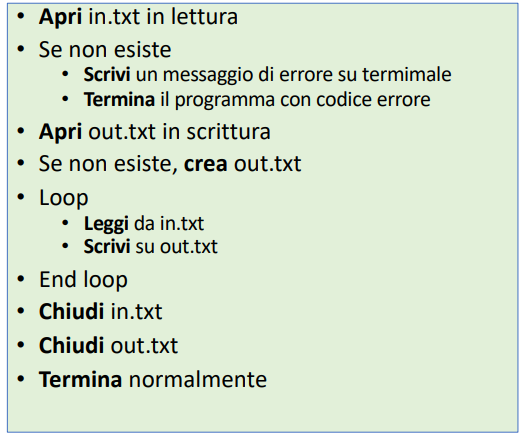
\includegraphics[width = 0.55\textwidth]{Images/9.PNG}
\end{center}
I programmi di sistema sono implementati utilizzando le API, esattamente come i programmi applicativi.
Consideriamo ad esempio il comando \textit{cp} delle shell dei sistemi operativi Unix-like; la sua sintassi è:
\begin{center}
    \textit{cp in.txt out.txt}
\end{center}
Esso copia il contenuto del file \textit{in.txt} in un file \textit{out.txt}. Se il file \textit{out.txt} esiste, il contenuto precedente viene cancellato, altrimenti \textit{out.txt} viene creato.
L'immagine sopra rappresenta una possibile struttura del codice; le invocazioni delle API sono riportate in grassetto.
\textit{cp} è implementato come programma di sistema.
\section{Processi e thread: i servizi}
Un sistema operativo esegue un certo numero di programmi sullo stesso sistema di elaborazione.
Il numero di programmi da eseguire può essere arbitrariamente elevato, di solito è infatti molto maggiore del numero di CPU del sistema.
A tale scopo, il sistema operativo realizza e mette a disposizione un'astrazione detta \textbf{processo}. Un processo è quindi un'entità attiva astratta definita dal sistema operativo allo scopo di eseguire un programma.
Per il momento, assumiamo che l'esecuzione di un processo sia sequenziale, tuttavia \textbf{rilasseremo presto questa assunzione}.
\subsection{Programmi e processi}
È fondamentale notare la differenza tra programma e processo!
\begin{itemize}
    \item Un programma è un'entità passiva (un insieme di istruzioni, tipicamente contenuto in un file sorgente o eseguibile)
    \item Un processo è un'entità attiva (è un \textbf{esecutore di un programma} o un \textbf{programma in esecuzione})
\end{itemize}
Uno stesso programma può dare origine a \textbf{diversi processi}:
\begin{itemize}
    \item Diversi utenti eseguono lo stesso programma
    \item Uno stesso programma viene eseguito più volte, anche contemporaneamente, dallo stesso utente
\end{itemize}
\subsection{Struttura di un processo}
Un processo è composto da diverse parti:
\begin{itemize}
    \item Lo stato dei registri del processore che esegue il programma, incluso il PC
    \item Lo stato della \textbf{immagine} del processo, ossia della regione di memoria centrale usata dal programma
    \item Le risorse del sistema operativo in uso al programma (files, locks, ...)
    \item Più diverse informazioni sullo stato del processo per il sistema operativo
\end{itemize}
Notare che processi distinti hanno immagini distinte! Due processi operano su zone di memoria centrale separate!
Le risorse del sistema operativo invece possono essere condivise tra processi (a seconda del tipo di risorsa)
\subsubsection{L'immagine di un processo}
L'intervallo di indirizzi di memoria in cui è contenuta l'immagine di un processo è anche detto \textbf{spazio di indirizzamento} (\textbf{address space}) del processo.
L'immagine di un processo di norma contiene:
\begin{itemize}
    \item \textbf{Text section}: contiene il codice macchina del programma
    \item \textbf{Data section}: contiene le variabili globali
    \item \textbf{Heap}: contiene la memoria allocata dinamicamente durante l'esecuzione
    \item \textbf{Stack delle chiamate}: contiene parametri, variabili locali e indirizzo di ritorno delle varie procedure che vengono invocate durante l'esecuzione del programma
\end{itemize}
\begin{center}
    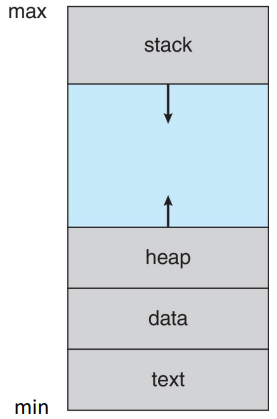
\includegraphics[width = 0.35\textwidth]{Images/10.PNG}
\end{center}
Text e data section hanno dimensioni costanti per tutta la vita del processo; mentre stack e heap invece crescono e decrescono durante la vita del processo.
\subsection{Operazioni sui processi}
I sistemi operativi di solito forniscono delle chiamate di sistema con le quali un processo può creare, terminare e manipolare altri processi.
Dal momento che solo un processo può creare un altro processo, all'avvio il sistema operativo crea dei processi \textbf{primordiali} dai quali tutti i processi utente e di sistema vengono progressivamente creati.
\subsubsection{Creazione di processi}
Di solito nei sistemi operativi i processi sono organizzati in maniera \textbf{gerarchica}:
Un processo \textbf{padre} può creare altri processi \textbf{figli} che a loro volta potranno essere i padri di nuovi processi.
Ciò va a creare un \textbf{albero di processi}
\begin{center}
    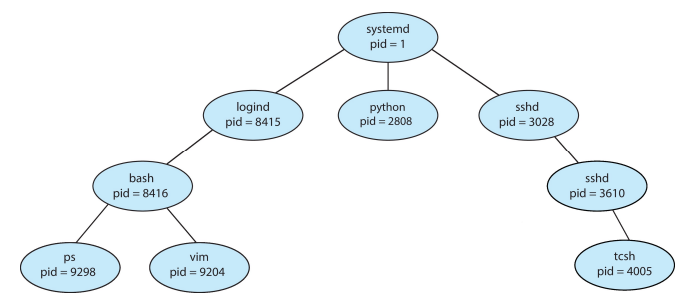
\includegraphics[width = 0.74\textwidth]{Images/11.PNG}
\end{center}
La relazione padre/figlio è di norma importante per le politiche di condivisione delle risorse e di coordinazione tra processi.
Vi sono diverse \textbf{politiche di condivisione di risorse}:
\begin{itemize}
    \item Padre e figlio condividono \textbf{tutte le risorse}...
    \item ...o un \textbf{opportuno sottoinsieme}...
    \item ...o \textbf{nessuna risorsa}
\end{itemize}
Quando un processo padre crea un processo figlio, esso può adottare diverse \textbf{politiche di creazione di spazio di indirizzi}:
\begin{itemize}
    \item Il figlio è un \textbf{duplicato} del padre (stessa memoria e programma1)...
    \item oppure no, e bisogna \textbf{specificare quale programma deve eseguire il figlio}
\end{itemize}
I processi padri e i loro figli possono inoltre \textbf{coordinarsi fra loro} seguendo delle \textbf{politiche di coordinazione padre/figli}:
\begin{itemize}
    \item Il padre è \textbf{sospeso} finché i figli non terminano...
    \item oppure eseguono in maniera \textbf{concorrente}
\end{itemize}
\subsubsection{Terminazione di processi}
I processi di regola richiedono esplicitamente la propria terminazione al sistema operativo. 
Un processo padre può attendere o meno la terminazione di un figlio oppure la \textbf{può forzare} per una serie di ragioni:
\begin{itemize}
    \item Il figlio sta usando \textbf{risorse in eccesso} (tempo, memoria, ...)
    \item Le funzionalità del figlio \textbf{non sono più richieste} (in questo caso, tuttavia, è meglio terminarlo in maniera ordinata tramite IPC)
    \item Il padre \textbf{termina prima del figlio} (in alcuni S.O.)
\end{itemize}
Riguardo all'ultimo punto, alcuni sistemi operativi \textbf{non permettono che i processi figli esistano se il loro processo padre è terminato}:
\begin{itemize}
    \item \textbf{Terminazione a cascata}: anche i nipoti, pronipoti, ecc... devono essere terminati
    \item La terminazione viene iniziata dal \textbf{sistema operativo}
\end{itemize}
\subsection{API POSIX per le operazioni sui processi}
\textbf{POSIX} (Portable Operating System Interface for Unix) è una famiglia di standard specificata dalla \textbf{IEEE} per mantenere la compatibilità del software tra diversi sistemi operativi,
in particolare tra le varianti di Unix (Linux e MacOS per esempio). In particolare definisce l'API disponibile (come la libreria \textbf{C POSIX} per il linguaggio C) e l'interfaccia a linea di comando
utilizzabile per shell (come \textbf{bash} e \textbf{dash}) e altri comandi fondamentali.
Un sistema operativo che segue gli standard POSIX si dice \textbf{POSIX-Compliant}.
Per operare sui processi, POSIX definisce le seguenti API:
\begin{itemize}
    \item \textbf{fork()}: Crea un nuovo processo figlio; il figlio è un duplicato del padre ed esegue concorrentemente ad esso; ritorna al padre un \textbf{numero identificatore} (PID) del processo figlio e al figlio il PID 0.
    \item \textbf{exec()}: Sostituisce il programma in esecuzione da un processo con un altro programma, che viene \textbf{eseguito dall'inizio}; viene tipicamente usato dopo una fork() dal figlio per iniziare ad eseguire un programma diverso da quello del padre.
    exec() tuttavia definisce un intera \textbf{famiglia di funzioni} in POSIX, ognuna distinta da dei \textbf{suffissi} di cui ogni lettera ha un significato particolare:
    \begin{itemize}
        \item \textbf{e}: Un \textbf{array di puntatori a variabili d'ambiente} è passato esplicitamente alla nuova immagine del processo
        \item \textbf{l}: Gli argomenti passati \textbf{da linea di comando} sono passati individualmente (come lista) alla funzione
        \item \textbf{p}: Utilizza la variabile d'ambiente \textbf{PATH} per trovare il file nominato nell'argomento "file" per eseguirlo
        \item \textbf{v}: Gli argomenti passati \textbf{da linea di comando} sono passati come un array di puntatori
    \end{itemize}
    Tendenzialmente, gli argomenti di una exec() sono:
    \begin{itemize}
        \item Il \textbf{path} del programma da eseguire oppure il \textbf{file descriptor} (fd) del file da eseguire
        \item Gli \textbf{argomenti} da passare all'entry point del programma da eseguire
    \end{itemize}
    \item \textbf{wait()}: viene chiamata dal padre per attendere la fine dell'esecuzione di un figlio; ritorna:
    \begin{itemize}
        \item il \textbf{PID} del figlio che è terminato
        \item Il codice di ritorno del figlio (passato come parametro dal figlio in \textbf{exit()})
    \end{itemize}
    \item \textbf{exit()}: fa terminare il processo che la invoca:
    \begin{itemize}
        \item Accetta come parametro un codice di ritorno numerico
        \item Il sistema operativo elimina il processo e recupera le sue risorse
        \item Quindi restituisce al processo padre il codice di ritorno (se ha invocato wait(), altrimenti lo memorizza per quando lo invocherà)
        \item Viene implicitamente invocata se il processo esce dalla funzione main
    \end{itemize}
    \item \textbf{abort()}: fa terminare forzatamente un processo figlio
\end{itemize}
Tendenzialmente la tipica sequenza di fork-exec è rappresentabile come segue:
\begin{center}
    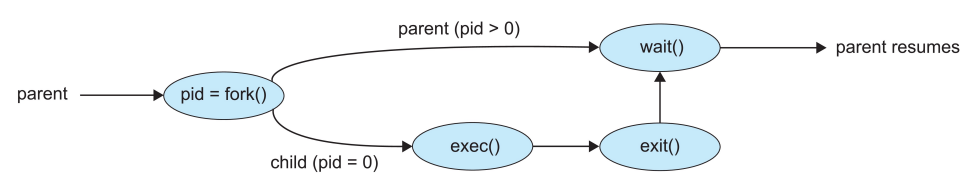
\includegraphics[width = 1\textwidth]{Images/12.PNG}
\end{center}
\subsection{Processi zombie e orfani}
Se un processo termina ma il suo padre non lo sta aspettando (cioè non ha invocato wait()), il processo è detto essere \textbf{zombie}:
le sue risorse non possono essere completamente deallocate (il padre potrebbe prima o poi invocare wait()).
Se un processo padre termina prima di un suo figlio e \textbf{non vi è terminazione a cascata} allora i suoi processi figli si dicono \textbf{orfani}.
\subsection{Comunicazione interprocesso}
Più processi possono essere indipendenti o cooperare. Un processo coopera con uno o più altri processi se il suo comportamento "influenza" o "è influenzato da" il comportamento di questi ultimi.
Vi sono più motivi per il quale si vogliono avere processi cooperanti:
\begin{itemize}
    \item \textbf{Condivisione} di informazioni
    \item \textbf{Accelerazione} di computazioni
    \item \textbf{Modularità} e \textbf{isolamento} (come in Chrome)
\end{itemize}
Per permettere ai processi di cooperare il sistema operativo deve mettere a disposizione primitive di \textbf{comunicazione interprocesso} (IPC).
Vi sono due tipi di primitive:
\begin{itemize}
    \item \textbf{Memoria condivisa}
    \item \textbf{Message passing}
\end{itemize}
\subsubsection{Modelli di IPC}
\begin{center}
    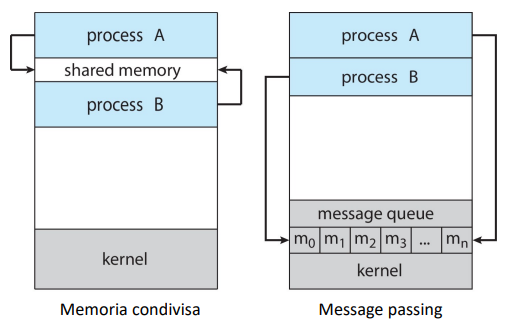
\includegraphics[width = 0.65\textwidth]{Images/13.PNG}
\end{center}
\subsubsection{IPC tramite memoria condivisa}
Nella IPC tramite memoria condivisa viene stabilita una zona di memoria condivisa tra i processi che intendono comunicare.
La comunicazione è \textbf{controllata dai processi che comunicano} e non dal sistema operativo.
Un problema importante è permette ai processi che comunicano tramite memoria condivisa di \textbf{sincronizzarsi} (un processo non deve leggere la memoria condivisa mentre l'altro sta scrivendo).
Allo scopo, i sistemi operativi mettono a disposizione ulteriori primitive per la \textbf{sincronizzazione}.
\subsubsection{IPC tramite message passing}
Nell'IPC tramite message passing, si permette ai processi \textbf{sia di comunicare che di sincronizzarsi}.
I processi comunicano tra di loro \textbf{senza condividere memoria} attraverso la mediazione del sistema operativo.
Questo mette a disposizione:
\begin{itemize}
    \item Un'operazione \textbf{send(message)} con la quale un processo può inviare un messaggio ad un altro processo
    \item Un'operazione \textbf{receive(message)} con la quale un processo può ricevere un messaggio o mettersi in attesa fino a quando non ne riceve uno.
\end{itemize}
Per comunicare fra loro, due processi devono:
\begin{itemize}
    \item Stabilire un \textbf{link di comunicazione} tra di loro
    \item Scambiarsi \textbf{messaggi} usando \textit{send} e \textit{receive}
\end{itemize}
\subsubsection{Pipe}
Le \textbf{pipe} sono canali di comunicazione tra i processi e sono una forma di IPC tramite \textbf{message passing}.
Ve ne sono di vario tipo:
\begin{itemize}
    \item \textbf{Unidirezionale}
    \item \textbf{Bidirezionale}
    \begin{itemize}
        \item \textbf{Half-Duplex}
        \item \textbf{Full-Duplex}
    \end{itemize}
    \item \textbf{Relazione} tra i processi comunicanti (sono padre-figlio oppure no)
    \item Usabili o meno in \textbf{rete}
\end{itemize}
Convenzionalmente, le pipe sono:
\begin{itemize}
    \item \textbf{Unidirezionali}
    \item Non accessibili al di fuori del processo creatore; sono quindi di solito \textbf{condivise} con un processo figlio attraverso una \textbf{fork()}
    \item In Windows sono chiamate \textbf{pipe anonime}
\end{itemize}
Vi sono anche le \textbf{named pipes}:
\begin{itemize}
    \item \textbf{Bidirezionali}
    \item Esistono anche \textbf{dopo la terminazione} del processo che le ha create 
    \item Non richiedono una relazione padre-figlio tra i processi che la usano
\end{itemize}
In \textbf{Unix}, le named pipes sono:
\begin{itemize}
    \item Half-duplex
    \item Sono accessibili solo sulla stessa macchina
    \item Trasportano solo dati byte-oriented
\end{itemize}
In \textbf{Windows} invece, le named pipes sono:
\begin{itemize}
    \item Full-duplex
    \item Sono accessibili anche da macchine diverse
    \item Trasportano anche dati message-oriented
\end{itemize}
\subsubsection{Notifiche con callback}
In alcuni sistemi operativi (es. API POSIX e Win32) un processo può \textbf{notificare} un altro processo in maniera da causare \textbf{l'esecuzione di un blocco di codice} ("callback"), similmente a 
ciò che avviene durante un \textbf{interrupt}.
Nei sistemi Unix-like (POSIX, Linux) tale notifiche vengono dette \textbf{segnali} ed interrompono in maniera \textbf{asincrona} la computazione del processo corrente,
causando un \textbf{salto brusco alla callback di gestione}, al termine della quale la computazione \textbf{ritorna al punto di interruzione}.
Nelle API Win32 esiste un meccanismo simile, detto \textbf{Asynchronous Procedure Call} (APC), che però richiede che il ricevente si metta \textbf{esplicitamente in uno stato di attesa} e che esponga un servizio che il mittente possa invocare.
\subsection{API POSIX per l'IPC}
\subsubsection{Memoria condivisa in POSIX}
Un processo crea o apre un segmento di memoria condivisa con la funzione \textit{smh\_open}:
\begin{center}
    \textit{int shm\_fd = shm\_open(const char *name, int oflag, mode\_t mode);}
\end{center}
dove:
\begin{itemize}
    \item Il parametro \textbf{oflag} può avere i seguenti valori:
    \begin{itemize}
        \item \textbf{O\_RDONLY}: Apertura in sola lettura
        \item \textbf{O\_RDWR}: Apertura per lettura o scrittura
        \item \textbf{O\_CREAT}: Crea lo spazio di memoria condivisa
        \item \textbf{O\_EXCL}: Se \textbf{O\_EXCL} e \textbf{O\_CREAT} sono settate; allora \textit{shm\_open} fallisce se l'oggetto di memoria condivisa con quel nome esiste già. Se invece Se \textbf{O\_EXCL} è settata ma non Se \textbf{O\_CREAT} allora il risultato è \textbf{indefinito}
        \item \textbf{O\_TRUNC}: Se l'oggetto esiste ed è stato aperto con successo tramite \textbf{O\_RDWR}, allora l'oggetto sarà troncato a lunghezza 0.
        \item Si possono utilizzare \textbf{O\_RDONLY} e \textbf{O\_RDWR} in combinazione con le altre flag, ma non insieme.
    \end{itemize}
    \item Il parametro \textit{mode} indica invece la \textbf{modalità di accesso} con cui si sta accedendo all'oggetto di memoria condivisa.
    La modalità è quindi con quali \textbf{permessi} si accede all'oggetto ed essi sono rappresentati da una \textbf{maschera di bit} in base 8 (da 0 a 7).
    In UNIX, i permessi sono rappresentati tramite \textbf{3 triadi}, che rappresentano rispettivamente quali permessi sul file hanno \textbf{l'utente, i membri del gruppo e gli utenti "esterni al gruppo"}.
    Diamo una tabella di quelli più comuni:
    \begin{center}
        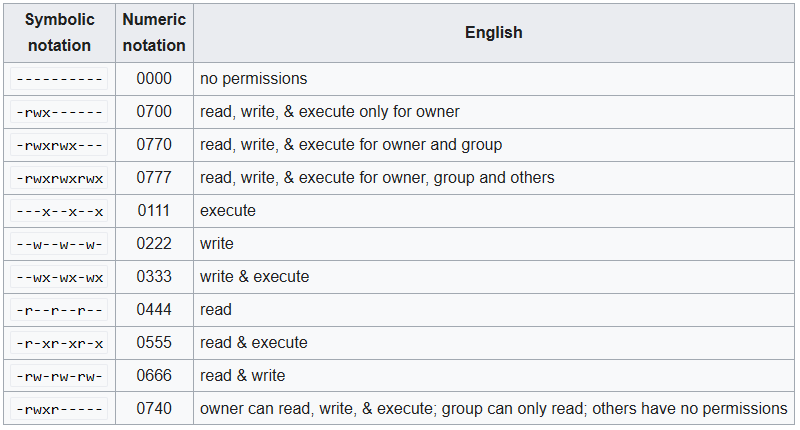
\includegraphics[width = 0.90\textwidth]{Images/14.PNG}
    \end{center}
\end{itemize}
Un esempio di chiamata è:
\begin{center}
    \textit{int shm\_fd = shm\_open(name, O\_CREAT | O\_RWDR, 0666)}
\end{center}
Quando si crea un nuovo segmento, è necessario \textbf{impostarne la dimensione}; ciò viene fatto tramite la funzione
\textbf{ftruncate} che ha firma:
\begin{center}
    \textit{int ftruncate(int fildes, off\_t length)}
\end{center}
Dove \textbf{fildes}, nel nostro caso, è il \textbf{file descriptor} del segmento di memoria e \textbf{length} sarà la dimensione
che gli vogliamo dare (in byte).
Infine, la funzione \textbf{mmap} mappa la memoria condivisa nello spazio:
\begin{center}
    \textit{void* mmap(void* addr, size\_t len, int prot, int flags, int fildes, off\_t off);}
\end{center}
dove:
\begin{itemize}
    \item Il parametro \textbf{addr} è l'indirizzo di partenza dello spazio di memoria condivisa. Questo parametro viene in verità usato come
    \textbf{SUGGERIMENTO} da parte del kernel del sistema operativo; ciò accade perché lo spazio di indirizzi indicato da addr e len \textbf{potrebbe essere già allocato}.
    \item Il parametro \textbf{length} specifica la lunghezza (in byte) dello spazio di memoria allocato
    \item Il parametro \textbf{prot} indica quali operazioni sono permesse sulla regione di memoria; esso può assumere:
    \begin{itemize}
        \item \textbf{PROT\_READ}: I dati possono essere letti
        \item \textbf{PROT\_WRITE}: I dati possono essere scritti
        \item \textbf{PROT\_EXEC}: I dati possono essere eseguiti
        \item \textbf{PROT\_NONE}: I dati non possono essere acceduti
    \end{itemize}
    \item Il parametro \textbf{flag} fornisce ulteriori informazioni riguardo la gestione dei dati mappati sullo spazio di memoria. Esso può assumere:
    \begin{itemize}
        \item \textbf{MAP\_SHARED}: I cambiamenti sono condivisi
        \item \textbf{MAP\_PRIVATE}: I cambiamenti sono privati
        \item \textbf{MAP\_FIXED}: Quando questa flag è impostata, la regione di memoria allocata \textbf{parte esattamente da addr} al posto di usarlo come un suggerimento.
    \end{itemize}
    \item Il parametro \textbf{fildes} indica il file (o l'oggetto) che rappresenta lo spazio di memoria condivisa
    \item Il parametro \textbf{off} indica l'offset nel file da dove inizia lo spazio di memoria condivisa
\end{itemize}
Un'esempio di chiamata può essere:
\begin{center}
    \textit{void* shm\_ptr = mmap(0, 4096, PROT\_WRITE, MAP\_SHARED, shm\_fd, 0)}
\end{center}
Da questo momento si può quindi usare il puntatore shm\_ptr ritornato da mmap per leggere/scrivere la memoria condivisa.
\subsubsection{Pipe anonime in POSIX}
Le pipe anonime in POSIX vengono create con la funzione \textit{pipe}, che ritorna due descrittori, uno per punto di lettura e uno per il punto di scrittura.
Ipotizziamo quindi di avere un array \textit{int pd\_fd[2]}; la funzione \textit{pipe} ha la seguente firma:
\begin{center}
    \textit{pipe(int fildes[2])}
\end{center}
Con \textit{fildes[2]} l'array in cui verranno scritti i descrittori di lettura e scrittura (lettura nella cella 0 e scrittura nella cella 1). La funzione ritorna 0 se ha avuto successo, -1 altrimenti; in questo caso
verrà impostata la flag \textit{ERRNO} per indicare l'errore e i descrittori NON verranno allocati all'interno di \textit{fildes[2]}. Un esempio di chiamata di \textit{pipe} è:
\begin{center}
    \textit{int res = pipe(p\_fd)}
\end{center}
Le funzioni \textit{read} e \textit{write} permettono rispettivamente di leggere e scrivere: \newline
La funzione write ha la seguente firma:
\begin{center}
    \textit{ssize\_t write (int fildes, const void* buf, size\_t nbyte)}
\end{center}
Essa cercherà di scrivere \textit{nbyte} dal buffer puntato da \textit{buf} al file associato al file descriptor \textit{fildes}.
La funzione ritorna il numero di byte effettivamente scritto, altrimenti -1.
Una scrittura sulla pipe anonima d'esempio può essere quindi:
\begin{center}
    \textit{ssize\_t n\_wr = write(p\_fd[1], "Hello World!", 14);}
\end{center}
La funzione \textit{read} ha la seguente firma:
\begin{center}
    \textit{ssize\_t read(int fildes, void* buf, size\_t nbyte);}
\end{center}
La funzione cercherà di leggere \textit{nbyte} dal file associato al file descriptor \textit{fildes} e di porre ciò che ha letto
nel buffer puntato da \textit{buf}. La funzione restituirà il numero di byte letti se ha avuto successo, -1 altrimenti.
Un esempio di lettura dalla pipe anonima d'esempio può essere quindi:
\begin{center}
    \textit{char buffer[256];} \\
    \textit{ssize\_t n\_rd = read(p\_fd[0], buffer, sizeof(buffer) - 1);}
\end{center}
\subsubsection{Named Pipes in POSIX}
Le named pipes vengono anche chiamate \textbf{FIFO} nei sistemi POSIX. Per creare una FIFO, si utilizza l'API \textit{mkfifo}, che ha la seguente firma:
\begin{center}
    \textit{int mkfifo(const char *path, mode\_t mode);}
\end{center}
La funzione andrà a creare un nuovo file speciale FIFO con nome dato dal percorso puntato da \textit{path}.
I bit dei permessi del file saranno impostati come specificato in \textit{mode}.
La funzione ritorna 0 se la creazione del file avviene con successo, -1 altrimenti.
Un esempio di chiamata può quindi essere:
\begin{center}
    \textit{int res = mkfifo("/home/pietro/myfifo", 0640);}
\end{center}
La FIFO quindi potrà utilizzare come un normale file; in particolare possiamo aprirla tramite l'API \textit{open}:
\begin{center}
    \textit{int open(const char *path, int oflag, ...);}
\end{center}
La funzione quindi aprirà il file specificato in \textit{path}.
Il parametro \textit{flag} deve obbligatoriamente assumere uno dei seguenti valori:
\begin{itemize}
    \item \textbf{O\_RDONLY}: il file viene aperto in modalità di sola lettura
    \item \textbf{O\_WRONLY}: il file viene aperto in modalità di sola scrittura
    \item \textbf{O\_RDWR}: Il fine viene aperto ed è possibile effettuare su di esso sia le operazioni di lettura che di scrittura
\end{itemize}
Inoltre è possibile specificare, in OR bitwise (|) con uno dei valori di \textit{flag} sopra (cioè viene fatto l'or bit a bit dei valori), le seguenti flag:
\begin{itemize}
    \item \textbf{O\_APPEND}: Il file viene aperto in "append mode", cioè ogni scrittura viene fatta alla fine del file
    \item \textbf{O\_CLOEXEC}: Viene impostata, per questo file, la flag \textbf{FD\_CLOEXEC}, cioè il file verrà chiuso se un processo che lo gestisce usa una delle funzioni della famiglia \textit{exec} viene eseguita sul file
    \item \textbf{O\_CLOFORK}: Viene impostata, per questo file, la flag \textbf{FD\_CLOFORK}, cioè il file verrà chiuso se un processo che lo gestisce effettua una \textit{fork()}
    \item \textbf{O\_CREAT}: Se il \textbf{path} non esiste, lo crea come un file normale. (n.d.a Si faccia riferimento a \textit{man} o alla documentazione POSIX per una spiegazione più dettagliata)
    \item \textbf{O\_DIRECTORY}: Se \textit{path} risolve a un file che NON è una directory, questa flag porta la funzione a fallire
    \item \textbf{O\_EXCL}: Se \textbf{O\_CREAT} e \textbf{O\_EXCL} sono entrambe impostate, la funzione fallirà se il file già esiste. Se invece solo questa flag è impostata, il risultato è \textbf{indefinito}
    \item \textbf{O\_TRUNC}: Se il file esiste ed è un file normale e il file è stato aperto con successo in modalità "sola scrittura" (flag ha valore \textit{O\_WRONLY}) oppure in è aperto in "modalità lettura e scrittura" (flag ha valore \textit{O\_RDWR}), allora tutti i contenuti del file verranno troncati (cioè cancellati) e la sua lunghezza verrà impostata a 0.
\end{itemize}
Quindi, un esempio di apertura di una FIFO può essere il seguente:
\begin{center}
    \textit{int fd = open("/home/pietro/myfifo", O\_RDONLY);}
\end{center}
Poiché una FIFO può essere utilizzata come un file normale, possiamo anche usare le API \textit{read} e \textit{write} viste prima per leggere e scrivere su di essa:
\begin{center}
    \textit{char buffer[256];} \\
    \textit{ssize\_t n\_rd = read(fd, buffer, sizeof(buffer) - 1);}
\end{center}
Al termine dell'utilizzo, dobbiamo ricordarci di \textbf{chiudere la FIFO}; per farlo usiamo l'API \textbf{close}:
\begin{center}
    \textit{int close(int fildes)}
\end{center}
La funzione prende in input il file descriptor e lo chiude (cioè chiude il file).
La funzione ritorna 0 se ha successo, -1 se invece fallisce. Per chiudere la FIFO che abbiamo presentato fino a qui come esempio,
possiamo quindi procedere in questo modo:
\begin{center}
    \textit{close(fd);}
\end{center}
Per invece \textbf{eliminare} una FIFO, possiamo usare l'API \textbf{unlink}:
\begin{center}
    \textit{int unlink(const char* path)}
\end{center}
l'API, in generale, si comporta in maniera differente in base a \textbf{cosa viene specificato come valore di path}:
\begin{itemize}
    \item Se quel nome era \textbf{l'ultimo collegamento ad un file e nessun processo ha quel file aperto}, il file viene \textbf{eliminato} e lo spazio che stava usando viene reso disponibile per il riuso.
    Se invece il file è ancora in uso da parte di un processo, esso rimarrà in memoria fino a quando \textbf{l'ultimo file descriptor che lo referenzia non viene chiuso}.
    \item Se il nome specificato è un \textbf{link simbolico} (un collegamento), esso viene rimosso
    \item Se il nome si riferisce ad una \textbf{Socket}, una \textbf{FIFO} o ad un \textbf{dispositivo}, allora il nome viene rimosso, ma i processi che lo stavano usando \textbf{possono continuare a farlo}
\end{itemize} 
La funzione ritorna 0 se ha successo, altrimenti -1. Per eliminare quindi una FIFO usando \textit{unlink}, possiamo procedere nel seguente modo:
\begin{center}
    \textit{unlink("/home/pietro/myfifo");}
\end{center}
\subsubsection{Segnali in POSIX}
Possiamo inviare un segnale ad un processo utilizzando l'API \textit{kill}:
\begin{center}
    \textit{int kill(pid\_t pid, int sig)}
\end{center}
Dove \textit{pid} è l'ID del processo e \textit{sig} è il segnale che si vuole inviare.
I segnali che si possono inviare sono definiti nella libreria \textbf{signal.h}.
Un esempio di utilizzo può essere il seguente:
\begin{center}
    \textit{int ok = kill(1000, SIGTERM);}
\end{center}
Per registrare una callback per un determinato segnale, possiamo usare l'API \textit{sigaction}:
\begin{center}
    \textit{int sigaction(int sig, const struct sigaction *restrict act, struct sigaction *restrict oact);}
\end{center}
In particolare, la funzione permette al processo chiamate di esaminare e/o specificare l'azione che deve essere associata ad un certo segnale.
Il parametro \textit{sig} specifica il segnale, i cui valori accettabili sono definiti in \textbf{signal.h}. La \textbf{struttura} sigaction, usata per
descrivere l'azione da intraprendere, è definita anch'essa in \textbf{signal.h} ed include almeno i seguenti membri:
\begin{center}
    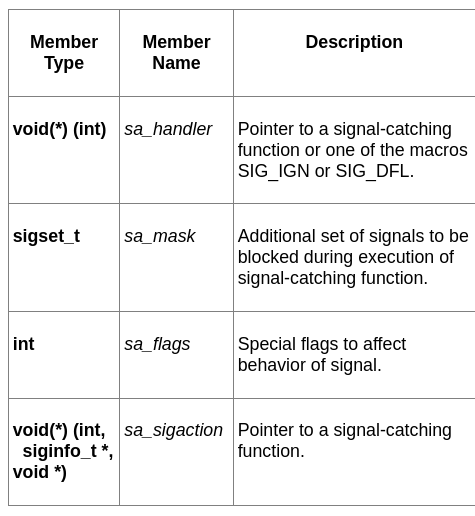
\includegraphics[width = 0.55\textwidth]{Images/15.PNG}
\end{center}
Abbiamo poi comportamenti diversi a seconda del valore degli argomenti \textit{act} e \textit{oact}. Per quanto
riguarda \textit{act} abbiamo:
\begin{itemize}
    \item Se il suo valore NON è un \textbf{puntatore a null}, esso punta ad una struttura che specifica l'azione da essere associata con il segnale specificato
    \item Se il suo valore È un \textbf{puntatore a null}, la gestione dei segnali \textbf{rimane invariata} (rispetto alla gestione normale del S.O.)
\end{itemize}
Per quanta riguarda \textit{oact} invece abbiamo:
\begin{itemize}
    \item Se il suo valore NON è un \textbf{puntatore a null}, l'azione precedentemente associata al segnale è immagazzinate nella locazione puntata da \textit{oact}
\end{itemize}
L'API restituirà 0 se ha avuto successo, -1 altrimenti.
Un esempio quindi di registrazione di una callback è il seguente:
\begin{center}
    \textit{struct sigaction act;} \\
    \textit{sigemptyset(\textnormal{\&}act.sa\_mask); /* non bloccare gli altri segnali */} \\
    \textit{act.sa\_flags = SA\_SIGINFO; /* callback in act.sa\_sigaction *()} \\
    \textit{act.sa\_sigaction = sigterm\_handler; /* la callback */} \\
    \textit{int ok = sigaction(SIGTERM, \textnormal{\&}act, NULL);}
\end{center}
\subsection{Multithreading}
Fino ad ora abbiamo assunto che un processo abbia un singolo flusso di esecuzione sequenziale (ossia, un singolo processore virtuale).
Se supponiamo che un processo possa avere \textbf{molti} processori virtuali, più istruzioni possono eseguire concorrentemente, e quindi il processo può avere più percorsi
(\textbf{thread}) di esecuzione concorrenti.
I thread di uno stesso processo condividono la memoria globale (data), la memoria contenente il codice (code) e le risorse ottenute dal sistema operativo (ad esempio i file aperti).
Ogni thread di uno stesso processo però deve avere \textbf{proprio stack}, altrimenti le chiamate a subroutine di un thread interferirebbero con quello di un altro thread concorrente.
\begin{center}
    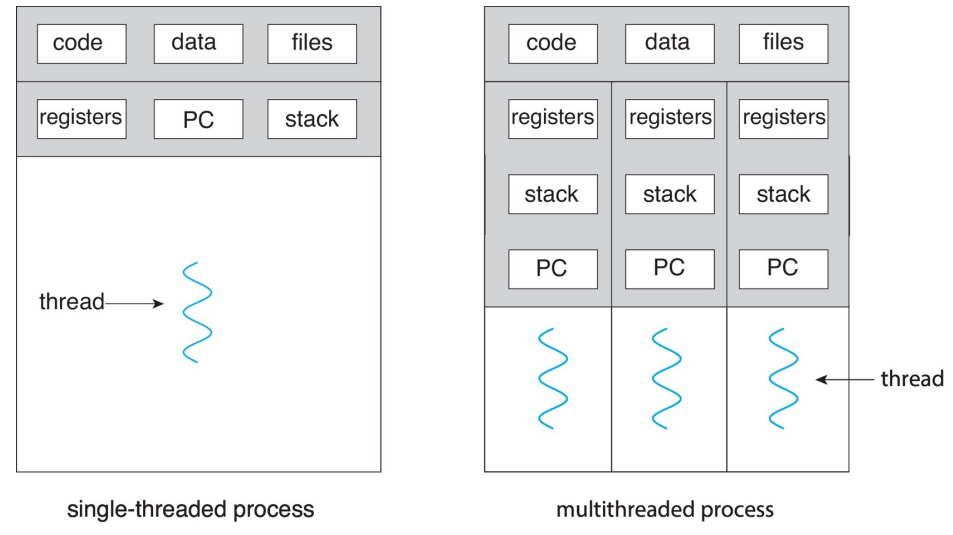
\includegraphics[width = 0.85\textwidth]{Images/16.PNG}
\end{center}
Le \textbf{librerie di un thread} sono le API fornite al programmatore per creare e gestire un thread.
Le librerie più in uso sono \textbf{POSIX pthreads} e \textbf{Windows Threads}.
\subsection{POSIX pthreads}
La libreria \textbf{POSIX pthreads non sono un'implementazione}, ma una specifica (POSIX standard IEEE 1003.1c).
Esse sono comuni nei sistemi Unix e Unix-like (BSD, Linux, MacOS).
All'inizio di un processo, viene creato un singolo thread.
Per creare un nuovo thread si utilizza l'API \textit{pthread\_create}, la quale ha la seguente firma:
\begin{center}
    \textit{pthread\_create(pthread\_t *restrict thread, const pthread\_attr\_t *restrict attr, void *(*start\_routine)(void*), void* restrict arg);}
\end{center}
L'API creerà un nuovo thread, con gli attributi specificati da \textit{attr}, all'interno del processo.
Se \textit{attr} è NULL, gli attributi di default saranno usati. Se gli attributi specificati da \textit{attr} sono vengono modificati successivamente, gli attributi
del thread creato non verranno modificati. Se l'esecuzione va a buon fine, l'API immagazzinerà l'ID del thread creato nella locazione specificata da \textit{thread}.
Il parametro \textit{start\_routine} indica \textbf{la funzione che il thread andrà ad eseguire}, passandogli \textbf{\textit{arg} come suo solo parametro}. Il thread continuerà ad eseguire fino a quando la funzione che sta eseguendo
non ritorna. La funzione \textit{pthread\_create} ritornerà 0 se ha successo, altrimenti verrà ritornato un numero diverso da 0 per indicare l'avvenimento di un errore.
Per invece attendere la fine dell'esecuzione di un thread si utilizza l'API \textit{pthread\_join}, la quale ha la seguente firma:
\begin{center}
    \textit{int pthread\_join(pthread\_t thread, void ** value\_ptr);}
\end{center}
L'API \textbf{sospenderà} l'esecuzione del thread chiamante fino a quando il thread obbiettivo (specificato nel parametro \textit{thread}) termina, a meno che il thread obbiettivo non sia già terminato.
Quando l'API ritorna con successo con un valore di \textit{value\_ptr} non NILL, il valore passato a \textit{pthread\_exit()} (API chiamata per cancellare un thread) dal thread terminante sarà reso disponibile
nella locazione referenziata da \textit{value\_ptr}.
L'API ritornerà 0 se la funzione ha successo, altrimenti sarà ritornato un numero diverso da 0 che indica l'errore.
Un esempio di utilizzo di queste due API può essere il seguente:
\begin{center}
    \textit{void* thread\_code(void* name) {...}} \\
    \textit{...} \\
    \textit{pthread\_id tid1, tid2;} \\
    \textit{int ok1 = pthread\_create(\textnormal{\&}td1, NULL, thread\_code, "thread 1);} \\
    \textit{int ok2 = pthread\_create(\textnormal{\&}td2, NULL, thread\_code, "thread 2);} \\
    \textit{...} \\
    \textit{void *ret1, *ret2;} \\
    \textit{ok1 = pthread\_join(tid1, \textnormal{\&}ret1);} \\
    \textit{ok2 = pthread\_join(tid2, \textnormal{\&}ret2);}
\end{center}
\newpage
\subsubsection{Comportamento rispetto alle chiamate di sistema fork() ed exec()}
Una \textit{fork()} dovrebbe duplicare solo il thread chiamante o tutti i thread? Alcuni sistemi operativi Unix-like hanno
\textbf{diverse \textit{fork()}}.\newline
\textit{exec()} invocata da un thread che effetto ha sugli altri thread? Di solito \textbf{termina tutti i thread del processo} precedentemente
all'esecuzione.
\subsubsection{Gestione dei segnali}
Quando un processo è single-threaded, un segnale interrompe l'unico thread del processo.
Quando vi sono più thread, quale thread riceve il segnale? Vi sono diversi soluzioni:
\begin{itemize}
    \item Il thread a cui si applica il segnale (ad es. il segnale \textit{SIGSEGV} viene inviato al thread che ha generato il segmentation fault)
    \item Ogni thread del processo
    \item Alcuni thread del processo
    \item Un thread speciale del processo deputato esclusivamente alla ricezione dei segnali
\end{itemize}
\subsubsection{Cancellazione dei thread}
L'operazione di cancellazione di un thread determina la terminazione prematura del thread.
Può essere invocata anche da un altro thread.
Vi sono due approcci per la cancellazione:
\begin{itemize}
    \item \textbf{Cancellazione asincrona}: il thread che riceve la cancellazione viene terminato immediatamente
    \item \textbf{Cancellazione differita}: un thread che supporta la cancellazione differita deve controllare periodicamente se esiste una richiesta di cancellazione pendente, e in tal caso terminare la propria esecuzione
\end{itemize}
Questi due approcci hanno i seguenti vantaggi:
\begin{itemize}
    \item \textbf{Cancellazione differita}: dal momento che un thread controlla il momento della propria cancellazione, può effettuare una terminazione ordinata
    \item \textbf{Cancellazione asincrona}: nessuna necessità di controllare periodicamente se ci sono richieste di cancellazione pendenti
\end{itemize}
Nei \textbf{POSIX pthreads} si può attivare/disattivare la cancellazione, ed avere sia cancellazione differita (default) che asincrona.
Se la cancellazione è inattiva, le richieste di cancellazione rimangono in attesa fino a quando (se) è attivata.
In caso di \textbf{cancellazione differita}, questa avviene solo quando l'esecuzione del thread raggiunge un punto di cancellazione (di solito una chiamata di sistema bloccante).
Il thread può aggiungere un punto di cancellazione controllando l'esistenza di richieste di cancellazione con la funzione \textit{pthread\_testcancel()}.
Presentiamo un esempio:
\begin{center}
    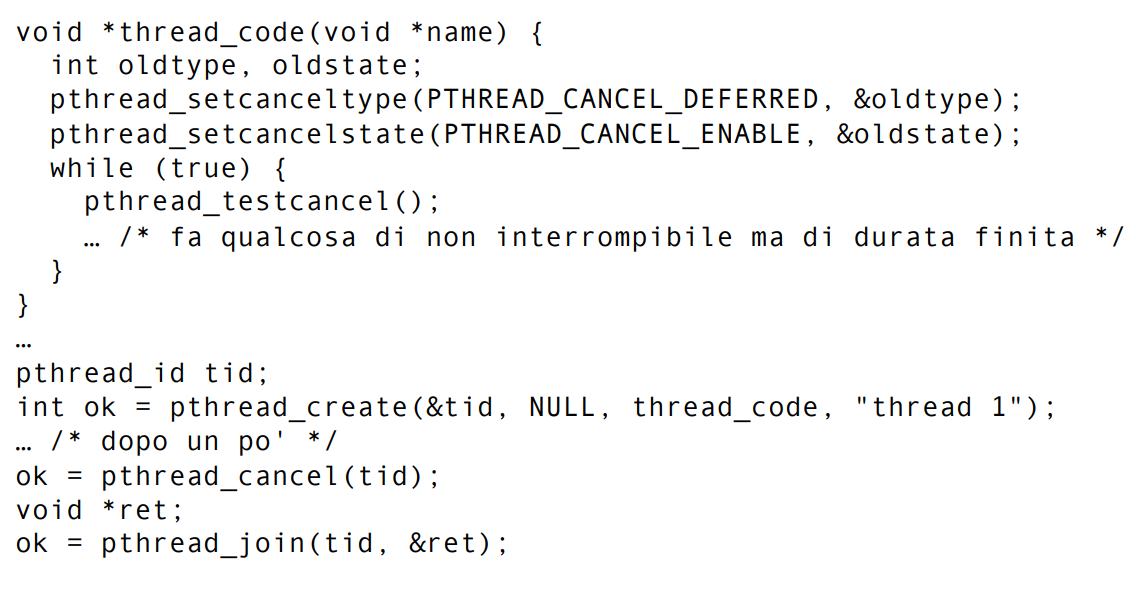
\includegraphics[width = 0.95\textwidth]{Images/17.png}
\end{center}
\subsubsection{Dati locali dei thread}
In alcuni casi è utile assegnare ad un thread dei dati locali (\textbf{thread local storage, TLS}) non condivisi con gli altri thread dello stesso processo.
La TLS è diversa dalle variabili locali (ad es. è visibile a tutte le funzioni). Essa è simile ai dati \textit{static} del linguaggio C, ma unica per ciascun thread. È utile quando il programma non ha un controllo
diretto sul momento di creazione dei thread (es. quando si usano i thread pools). In POSIX, i dati locali dei thread si possono creare utilizzando le funzioni:
\begin{itemize}
    \item \textbf{\textit{pthread\_key\_create(...)}}: crea un oggetto opaco di tipo \textit{pthread\_key\_t}, che può essere usato da tutti i thread per identificare un dato locale
    \item \textbf{\textit{pthread\_set\_specific(...)}}: permette di associare ad una \textit{pthread\_key\_t} un valore di tipo \textit{void*}
    \item \textbf{\textit{pthread\_getspecific(...)}}: permette di richiamare un oggetto \textit{pthread\_key\_t} data la chiave
\end{itemize} 
Ogni thread pul associare ad una stessa chiave il proprio distinto valore locale (e successivamente richiamarlo).

\section{Gestione della memoria: i servizi}
Perché un programma possa andare in esecuzione esso deve avere a disposizione:
\begin{itemize}
    \item Il processore, per eseguire il codice
    \item La memoria centrale, per memorizzare il codice e i dati sul quale il codice opera
\end{itemize}
Solo nei sistemi operativi più semplici un solo programma alla volta è in memoria: nei moderni sistemi operativi molti programmi sono contemporaneamente in memoria in uno stesso istante.
Secondo la terminologia precedentemente introdotta: più immagini di più processi sono presenti contemporaneamente nella memoria centrale.
Il sistema operativo deve, pertanto, allocare porzioni di memoria centrale ai diversi processi in funzione delle necessità di tali processi.
\subsection{Lo spazio di indirizzamento}
Ogni processo ha disposizione uno spazio di indirizzamento che può usare per le proprie operazioni.
\begin{center}
    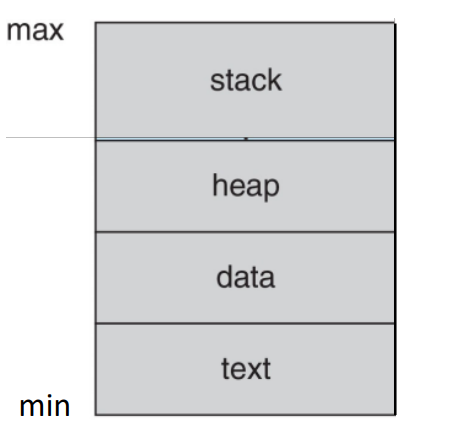
\includegraphics[width = 0.35\textwidth]{Images/18.png}
\end{center}
Nei primi sistemi operativi, tale spazio di indirizzamento era il range di indirizzi di memoria centrale che veniva assegnato al processo:
ad esempio, se l'immagine di un certo processo avesse avuto dimensione 1 MB e fosse stata caricata in memoria centrale dall'indirizzo 001B:000... il suo spazio di indirizzamento sarebbe
stato 001B:0000 - 002B:0000. Questo però non permette di caricare lo stesso programma in zone diverse della memoria!
\subsection{Associazione degli indirizzi}
In presenza di molti programmi in memoria, il sistema operativo di regola carica uno stesso programma, in momenti diversi, in diverse aree di memoria (dove trova spazio).
Come fa, pertanto, un'istruzione macchina di un programma afar riferimento ad una certa locazione di memoria, se il suo indirizzo non è noto a priori, ma dipende da dove il programma viene caricato?
Una prima possibilità è che il compilatore produca codice indipendente dalla posizione, ossia \textbf{position-independent code (PIC)}, ossia codice macchina che usi solo indirizzi di memoria \textbf{relativi}, e che quindi
funzioni correttamente in qualsiasi locazione di memoria venga caricato. Una seconda possibilità è produrre codice dipendente dalla posizione e tradurre gli indirizzi dipendenti dalla posizione negli indirizzi corretti.
Questa operazione di "traduzione" è detta di \textbf{associazione (binding) degli indirizzi}.
\subsubsection{Loader e Linker}
Un programma sorgente è compilato in un file oggetto che deve poter essere caricato a partire da qualsiasi locazione di memoria fisica (\textbf{file oggetto rilocabile}).
I \textbf{linker}, o linkage editor, combinano più file oggetto (diversi file sorgente + librerie) per formare un file eseguibile. I \textbf{loader} si occupano di caricare in memoria i file eseguibili nel momento
on cui devono essere eseguiti. Inoltre, i loader (o ulteriori linker dinamici) effettuano il linking delle \textbf{librerie dinamiche}
\begin{center}
    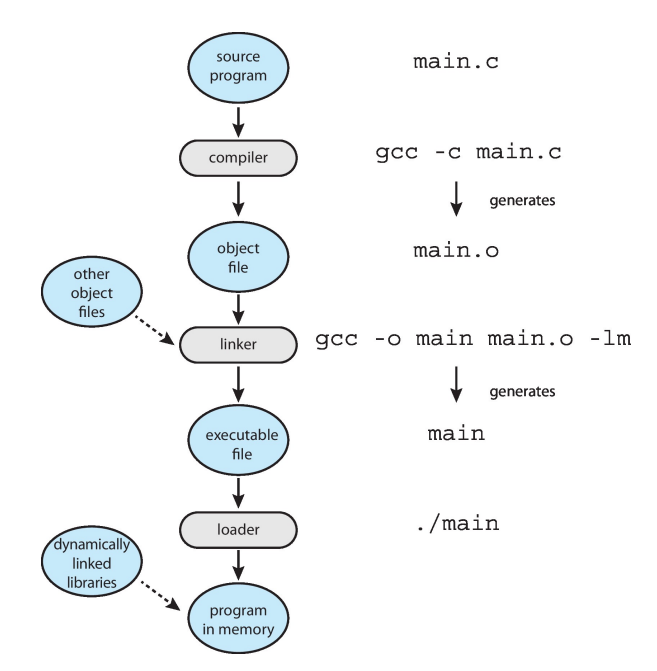
\includegraphics[width = 0.55\textwidth]{Images/19.png}
\end{center}
\subsubsection{Librerie dinamiche}
Nei sistemi operativi odierni, non tutto il linking viene fatto a compile time: le librerie dinamiche vengono collegate a quando il programma \textbf{caricato o durante l'esecuzione del programma stesso}.
Il vantaggio delle librerie dinamiche è che queste possono essere condivise tra diversi programmi, riducendo le dimensioni dei programmi stessi e risparmiando memoria.
\subsubsection{Varianti nell'associazione degli indirizzi}
L'associazione degli indirizzi può essere fatta in tre momenti diversi:
\begin{itemize}
    \item \textbf{In compilazione}: il linker, a partire dall'indirizzo di caricamento, effettua il binding e genera \textbf{codice assoluto}
    \item \textbf{In caricamento}: il linker genera \textbf{codice rilocabile} e il loader, a partire dall'indirizzo di caricamento, effettua il binding al momento del caricamento in memoria del codice
    \item \textbf{In esecuzione}: il binding viene effettuato dall'hardware dinamicamente mentre il codice viene eseguito
\end{itemize}
Questi approcci hanno sia \textbf{vantaggi e svantaggi}:
\begin{itemize}
    \item \textbf{In compilazione}: soluzione semplice, ma se cambia l'indirizzo di caricamento il codice va ricompilato (si possono, ad esempio, avere $n$ versioni per $n$ diversi indirizzi di caricamento)
    \item \textbf{In caricamento}: permette di variare liberamente l'indirizzo di caricamento da esecuzione ad esecuzione, ma è una soluzione lenta che non permette di rilocare (spostare) l'immagine di un processo durante la sua
    esecuzione; inoltre l'eseguibile deve contenere delle opportune tabelle che indichino le istruzioni macchina da modificare
    \item \textbf{In esecuzione}: soluzione rapida che permette di rilocare l'immagine di un processo anche durante la sua esecuzione, e di proteggere la memoria centrale non assegnata ad un processo, ma richiede il supporto dell'hardware
\end{itemize}
Il binding in esecuzione è quello di fatto usato in tutti i sistemi operativi moderni; il binding in compilazione è usato per \textbf{alcuni eseguibili speciali, come il kernel}, di cui si sa a priori l'indirizzo di caricamento.
\subsection{Spazio di indirizzamento virtuale}
Nei sistemi operativi moderni, ogni processo ha uno \textbf{spazio di indirizzamento virtuale}, o \textbf{virtual address space (VAS)} indipendente dagli indirizzi fisici della memoria centrale nella quale l'immagine è caricata.
\begin{center}
    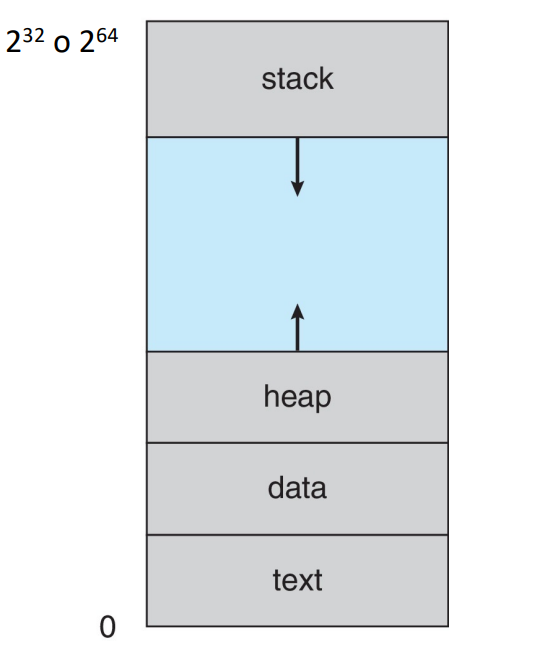
\includegraphics[width = 0.35\textwidth]{Images/20.png}
\end{center}
\begin{center}
    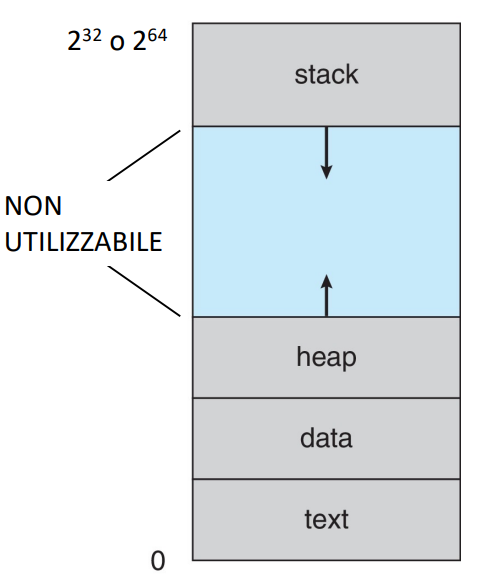
\includegraphics[width = 0.35\textwidth]{Images/21.png}
\end{center}
\noindent
Tale spazio di indirizzamento si estende dall'indirizzo 0 al massimo indirizzo consentito dall'architettura del processo.
Delle \textbf{tecniche di associazione degli indirizzi in esecuzione} fanno corrispondere lo spazio di indirizzamento virtuale del processo
con la regione (o le regioni) di memoria centrale che la sua immagine occupa.
Lo spazio di indirizzamento virtuale di un processo è di regola \textbf{molto più ampio della memoria centrale}.
Questo implica che buona parte dello spazio di indirizzamento virtuale \textbf{non è utilizzabile dal processo} perché non è associato a nessuna regione di memoria
centrale. Tale parte inutilizzabile è di solito compresa tra stack e heap. Stack e heap possono essere dinamicamente estesi e ridotti (automaticamente lo stack, attraverso le API lo heap).
\subsubsection{Librerie dinamiche}
Le librerie dinamiche vengono caricate nella zona tra stack e heap. Dal momento che possono essere caricate in qualsiasi posizione nel VAS, devono essere \textbf{compilate come PIC}.
\begin{center}
    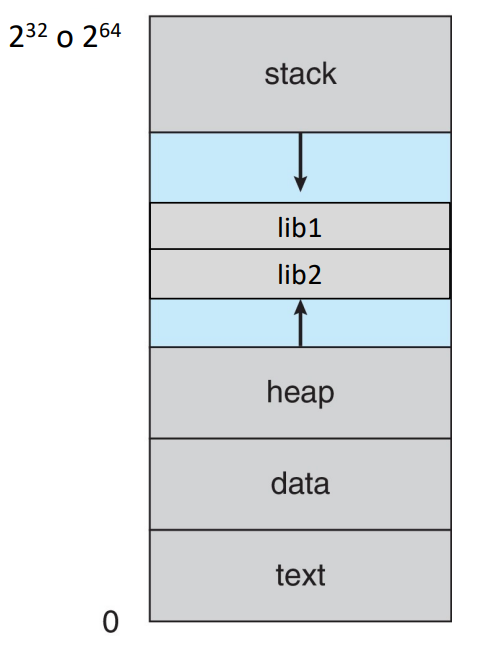
\includegraphics[width = 0.35\textwidth]{Images/22.png}
\end{center}
\subsubsection{Memory mapping}
\begin{center}
    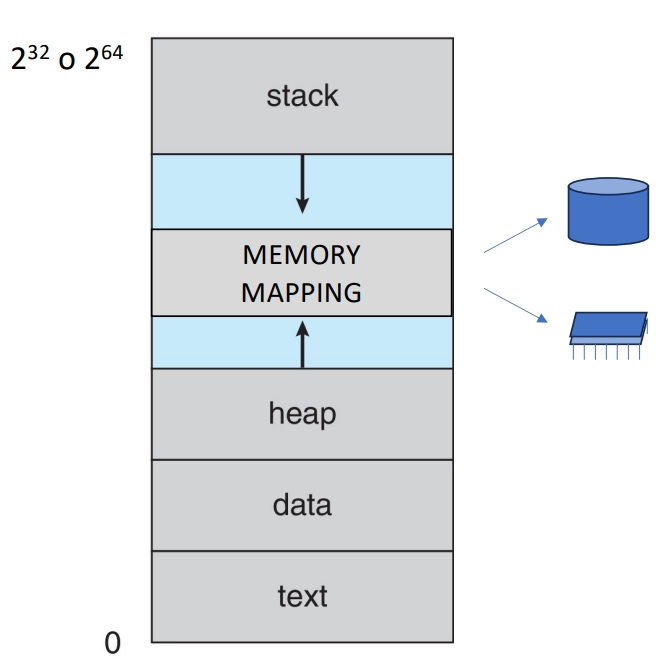
\includegraphics[width = 0.35\textwidth]{Images/23.png}
\end{center}
In generale, i sistemi operativi mettono a disposizione API per mappare una regione inutilizzabile del VAS su memoria centrale, così che diventi utilizzabile.
Esistono anche API che permettono di mappare una regione del VAS sul contenuto di un file (file mappati in memoria).
In tal modo l'accesso al file può avvenire utilizzando le istruzioni macchina per accedere alla memoria, anziché le API del filesystem.
\subsection{Le API POSIX per la gestione della memoria}
Di norma non dobbiamo usare le API per gestire stack e heap:
\begin{itemize}
    \item Lo stack è gestito automaticamente dal sistema operativo, non tramite API
    \item Lo heap è gestito di norma dal supporto runtime del linguaggio (new in C++) o dalla sua libreria (malloc in C), che \textbf{invocano API} per ridurre/espandere lo heap in funzione
    delle necessità del processo
\end{itemize}
Perché allora ci interessa sapere quali sono le API per la gestione della memoria?
\begin{itemize}
    \item Ci permettono di avere regioni di memoria con \textbf{permessi particolari} (sola lettura, eseguibili...)
    \item Ci permettono di implementare componenti quali allocatori di memoria, compilatori just-in-time,... qualora volessimo implementare il nostro nuovo linguaggio di programmazione
    \item Ci permettono di utilizzare i file mappati in memoria e la memoria condivisa
\end{itemize}
Le API Unix legacy per cambiare la dimensione del segmento dati (che nello standard POSIX comprende le regioni data e heap) sono \textit{brk} e \textit{sbrk}.
Tali API sono deprecate in favore dell'API \textit{mmap} (già presentata in questi appunti), e incompatibili con questa (ma esistono ancora in diversi OS, ad esempio Linux).
L'API mmap permette di mappare una regione ancora non utilizzata del VAS su:
\begin{itemize}
    \item \textbf{Memoria centrale}
    \item \textbf{Un file} (che viene mappato in memoria)
    \item \textbf{Memoria condivisa}
\end{itemize}
Vediamo un'ulteriore API per la gestione della memoria: \textit{msync}:
\begin{center}
    \textit{int msync(void* addr, size\_t len, int flags);}
\end{center}
L'API andrà a scrivere sul filesystem tutti i dati modificati in un file mappato in memoria 
da \textit{mmap}. Senza l'uso di questa funzione, non c'è garanzia che i cambiamenti scritti sul file
in memoria vengano mantenuti. Per essere più precisi, la parte del file che corrisponde all'area di memoria che
inizia a \textit{addr} e avente lunghezza \textit{len} viene aggiornata. L'attributo flag può avere i seguenti valori:
\begin{itemize}
    \item \textbf{MS\_ASYNC}: La scrittura delle modifiche viene effettuata in maniera asincrona
    \item \textbf{MS\_SYNC}: La scrittura delle modifiche viene effettuata in maniera sincrona
    \item \textbf{MS\_INVALIDATE}: Viene richiesto di invalidare altra mappature dello stesso file, così che possano essere aggiornate con i valori appena scritti
\end{itemize}
Queste flag sono definite in \textit{<sys/mman.h>} e possono essere combinate con un \textbf{bitwise-inclusive OR} (|).
La funzione ritorna 0 se ha successo, -1 altrimenti.
Vediamo un esempio di utilizzo di queste API:
\begin{center}
    \textit{// Mappiamo 4 KB di memoria a partire dall'indirizzo virtuale 0xa0000000} \\
    \textit{void* ptr = mmap(0xa0000000, 4096, PROT\_READ | PROT\_WRITE, MAP\_ANONYMOUS, 0, 0);} \\
    \textit{// Per mappare, a partire dall'indirizzo virtuale 0xb0000000, 8192 bytes del file /usr/foo a partire dal byte 100 scriviamo:} \\
    \textit{int fd = open("/usr/foo", O\_RDWR);} \\
    \textit{void* ptr = mmap(0xb0000000, 8192, PROT\_READ | PROT\_WRITE, MAP\_PRIVATE, fd, 100);} \\
    \textit{// Per sincronizzare le modifiche in memoria con il file, scriviamo:} \\
    \textit{int ok = msync(0xb0000000, 8192, MS\_SYNC|MS\_INVALIDATE);}
\end{center}
\section{File system: i servizi}
Il \textbf{file system} è il modo attraverso il quale il sistema operativo memorizza in linea i dati e i programmi.
Esso è costituito da:
\begin{itemize}
    \item Un insieme di file
    \item Una struttura delle directory, che organizza i file
\end{itemize}
Un \textbf{file} è una unità di memorizzazione logica, un insieme di informazioni correlate, registrare in memoria secondaria, alle quali è \textbf{stato dato un nome}.
Un file a sua volta è costituito da una \textbf{sequenza di record, righe, bit o byte}, il cui significato è definito dal creatore del file.
Un file possiede i seguenti attributi:
\begin{itemize}
    \item \textbf{Nome}: è di solito l'unica informazione in forma umanamente leggibile
    \item \textbf{Identificatore}: un'etichetta unica fornita dal file system per distinguere i file
    \item \textbf{Tipo}: tpo di dati contenuti nel file (alcuni S.O. non hanno questo attributo)
    \item \textbf{Locazione}: dispositivo di memoria secondaria e posizione nel dispositivo dove l'informazione del file è memorizzata
    \item \textbf{Dimensione}: in byte, parole, record, ...
    \item \textbf{Protezione}: informazione di controllo accessi
    \item \textbf{Ora, data e utente} che ha creato, letto o modificato per ultimo il file
    \item \textbf{Attributi estesi}: checksum, codifica caratteri, applicazioni correlate ecc...
\end{itemize}
Le informazioni sul file sono memorizzate nelle \textbf{directory}.
\subsection{Operazioni dei processi sui file}
I processi possono effettuare le seguenti operazioni sui file:
\begin{itemize}
    \item \textbf{Creazione}: viene riservato spazio nel file system per i dati, e viene aggiunto un elemento nella directory
    \item \textbf{Apertura}: effettuata prima dell'utilizzo del file
    \item \textbf{Lettura}: a partire dalla posizione determinata da un puntatore di lettura
    \item \textbf{Scrittura}: a partire dalla posizione determinata da un puntatore di scrittura (di solito coincide con il puntatore di lettura)
    \item \textbf{Riposizionamento (seek)}: spostamento del puntatore all'interno del file
    \item \textbf{Chiusura}: effettuata alla fine dell'utilizzo del file
    \item \textbf{Cancellazione e troncamento}: il troncamento canella i dati \textbf{ma non il file} con i suoi attributi
\end{itemize}
\subsection{Lock dei file}
Uno stesso file può essere aperto \textbf{contemporaneamente da più processi che operano in concorrenza}.
Alcuni sistemi operativi permettono di associare ai file (o a porzioni di esso) dei \textbf{lock} per coordinare i processi che operano sullo stesso file.
Vi sono due tipi di lock:
\begin{itemize}
    \item \textbf{Lock condiviso}: detto anche \textbf{lock di lettura}; più processi possono acquisirlo, proibisce l'acquisizione di un lock esclusivo
    \item \textbf{Lock esclusivo}: detto anche \textbf{lock di scrittura}; solo un processo alla volta può acquisirlo, proibisce l'acquisizione di un lock condiviso
\end{itemize}
Altre possibilità sono:
\begin{itemize}
    \item \textbf{Lock obbligatori (mandatory)}: il sistema operativo proibisce l'accesso al file ai processi che \textbf{non detengono il lock}
    \item \textbf{Lock consultivi (advisory)}: il sistema operativo \textbf{offre il lock} ma non regola l'accesso al file: sono i processi che devono evitare di accedere al file se non hanno il lock
\end{itemize}
I sistemi \textbf{Windows} adottano i lock obbligatori, i sistemi \textbf{Unix-life} i lock consultivi.
\subsection{Tipi di file}
Vi sono principalmente due tipi di file:
\begin{itemize}
    \item Dati (numerici, testo, binari)
    \item Programmi
\end{itemize}
Il sistema operativo può essere più o meno consapevole del tipo di file, \textbf{ma deve almeno riconoscere il tipo di file eseguibile}.
Possibili tecniche per riconoscere il tipo di file sono:
\begin{itemize}
    \item Schema del nome (nome.estensione)
    \item Attributi nel file (ad esempio in macOS, viene registrato il programma che ha creato il file)
    \item "Magic Number" all'inizio del file (ad esempio la "shebang" magic cookie ("\#!") all'inizio degli script Unix)
\end{itemize}
\subsection{Struttura dei file}
I file possono avere o meno una struttura ben definita; alcune possibilità sono:
\begin{itemize}
    \item Nessuna struttura (ad esempio, nei sistemi Unix-like un file è una sequenza di byte)
    \item \textbf{Sequenza di record} (righe di testo o record binari, a struttura e lunghezza fissa o variabile)
    \item \textbf{Strutture più complesse e standardizzate}, sopratutto per i file eseguibili (formato PE in Windows, a.out ed ELF nei sistemi Unix-like, Mach-O in macOS)
\end{itemize}
Più il sistema operativo supporta direttamente diverse strutture di file, \textbf{più diventa complesso}.
Inoltre se il sistema operativo è troppo "rigido" sulle possibili strutture, potrebbe non supportare nuovi tipi, o tipi \textbf{ibridi}.
\subsection{Metodi di accesso a file}
Vediamo ora quali possono essere i principali metodi di accesso ad un file
\subsubsection{Accesso sequenziale}
In questo tipo di accesso, il file \textbf{è una sequenza di record a lunghezza fissa}
\begin{center}
    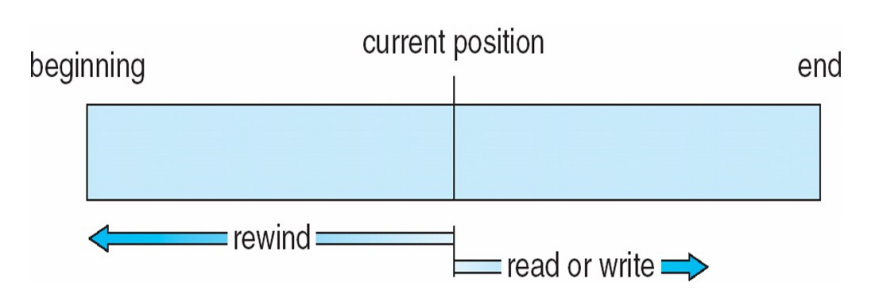
\includegraphics[width = 0.50\linewidth]{Images/24.png}
\end{center}
Le operazioni disponibili in questo caso sono:
\begin{itemize}
    \item \textit{read\_next()} e \textit{write\_next()} leggono/scrivono il successivo record dalla posizione corrente
    \item Operazione di \textbf{riavvolgimento}
\end{itemize}
\subsubsection{Accesso diretto}
In questo tipo di accesso, abbiamo a disposizione le seguenti operazioni:
\begin{itemize}
    \item Operazioni \textit{read(n)} e \textit{write(n)} per accedere direttamente all'n-esimo record
    \item Alternativamente, possiamo usare \textit{read\_next(), write\_next()} e \textit{position(n)}
\end{itemize}
\subsubsection{Accesso indicizzato}
In alcuni sistemi operativi, ad esempio quelli per mainframe IBM, i file possono essere \textbf{sequenze di record ordinate secondo un determinato campo chiave del record}.
In tali sistemi, l'accesso può essere basato \textbf{sulla chiave}, e il sistema operativo mantiene un indice per velocizzare l'accesso. Esempio è \textbf{l'accesso ISAM} (Indexed Sequential Access Method) nei sistemi IBM,
file systems \textbf{Files-11} prodotto da Digital per il sistema operativo OpenVMS (offre tutti e tre i tipi di accesso su record a lunghezza fissa o variabile).
\subsection{Directories}
Una \textbf{directory} è, in pratica, un elenco di file presenti nel file system.
Più formalmente, \textbf{è una tabella} che permette di associare il nome di un file ai dati (e metadati) contenuti nel file stesso.
Sia i file che le directory risiedono sul disco: deve esservi \textbf{almeno una directory nel file system} (altrimenti non sarebbe possibile ritrovare i file!)
I processi possono effettuare le seguenti operazioni sulle directory:
\begin{itemize}
    \item \textbf{Creazione} di un file in una directory
    \item \textbf{Cancellazione} di un file in una directory
    \item \textbf{Ridenominazione} di un file o \textbf{spostamento} da una directory ad un'altra
    \item \textbf{Elenco} dei file in una directory
    \item \textbf{Ricerca} di un file: basata sul nome, o suno schema di possibili nomi
    \item \textbf{Attraversamento} del file system, ad esempio per effettuare un backup
\end{itemize}
Le directories possono avere diversi tipi di struttura:
\begin{itemize}
    \item Ad un livello
    \item A due livelli
    \item Ad albero
    \item A grafo aciclico
    \item A grafo generale
\end{itemize}
\subsubsection{Struttra delle directory ad un livello}
\begin{center}
    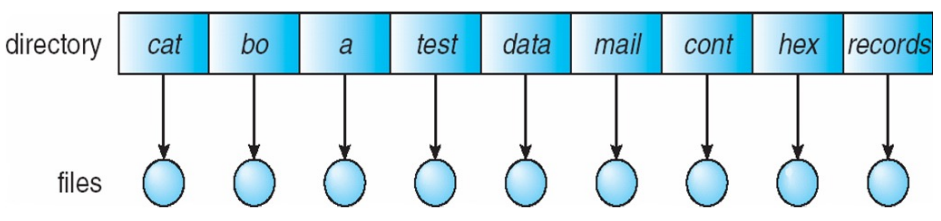
\includegraphics[width = 0.60\linewidth]{Images/25.png}
\end{center}
Nella struttura ad un livello, \textbf{esiste una sola directory per tutti i file}.
Il vantaggio di questa struttura è la \textbf{semplicità}, tuttavia ha diversi svantaggi:
\begin{itemize}
    \item Difficoltà nel nominare i file quando sono molti
    \item Difficoltà nel raggruppare i file per utenti diversi
\end{itemize}
\subsubsection{Struttura delle directory a due livelli}
\begin{center}
    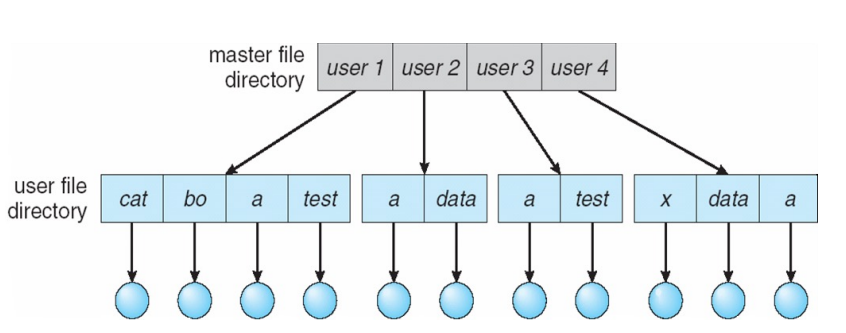
\includegraphics[width = 0.70\linewidth]{Images/26.png}
\end{center}
Nella struttura a due livelli, la directory principale \textbf{contiene delle sottodirectory, una per ogni utente}.
La sottodirectory utente contiene i \textbf{file dell'utente}; utenti diversi possono quindi dare \textbf{lo stesso nome a file diversi}.
Occorre quindi usare dei \textbf{nomi di percorso (path name)} per identificare un file univocamente:
\begin{itemize}
    \item \textit{/user2/data} (separatori Unix-like)
    \item \textit{\textbackslash user2 \textbackslash data} (separatori Windows like)
    \item \textit{>user2>data} (separatori MULTICS-like)
\end{itemize}
I file di sistema sono di solito posti \textbf{in una o più directory speciali}, e occorre che il sistema conosca un \textbf{percorso di ricerca} per trovarli.
\subsubsection{Struttura delle directory ad albero}
\begin{center}
    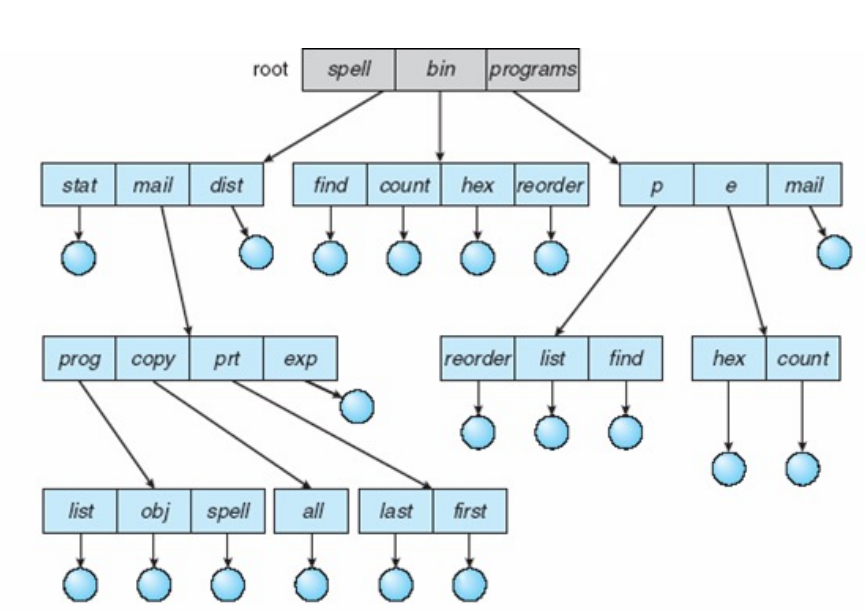
\includegraphics[width = 0.60\linewidth]{Images/27.png}
\end{center}
Nella struttura ad albero, ogni directory \textbf{contiene ricorsivamente files e altre directory}. Questa struttura quindi
permette agli utenti di \textbf{raggruppare i propri file}. Per semplificare l'accesso, ad ogni programma è assegnata una \textbf{directory corrente}, dalla quale si possono specificare
\textbf{path relativi}
\begin{itemize}
    \item Esempio: se la directory corrente è \textit{/programs/mail}, un path relativo potrebbe essere \textit{prt/first}
\end{itemize}
In questo caso, come avviene la cancellazione della directory?
\begin{itemize}
    \item Con la directory \textbf{cancello tutto il suo contenuto}
    \item Oppure permetto di cancellare una directory \textbf{solo se è vuota}. Questa soluzione è la più sicura
\end{itemize}
\subsubsection{Struttra delle directory a grafo aciclico}
\begin{center}
    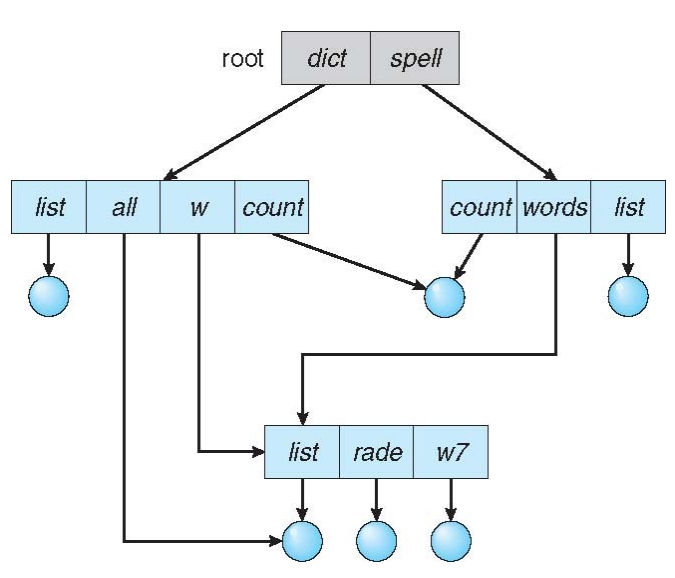
\includegraphics[width = 0.50\linewidth]{Images/28.png}
\end{center}
La struttura a grafo aciclico \textbf{permette l'aliasing} (più di un nome per lo stesso file).
Cosa succede però se \textbf{cancello un file/directory con un alias?}
\begin{itemize}
    \item \textbf{Hard links}: duplicazione voci di directory; viene introdotto un \textbf{contatore} ai riferimenti, quando è a zero viene \textbf{cancellato il file}
    \item \textbf{Link simbolici}: riferimenti simbolici ad un \textbf{path assoluto}, quando questo è cancellato restano \textbf{dangling}; non sono aggiunti al contatore dei riferimenti
\end{itemize}
Questo tipo di struttura delle directory introduce anche un \textbf{problema di attraversamento del file system}.
\subsubsection{Struttura delle directory a grafo generico}
\begin{center}
    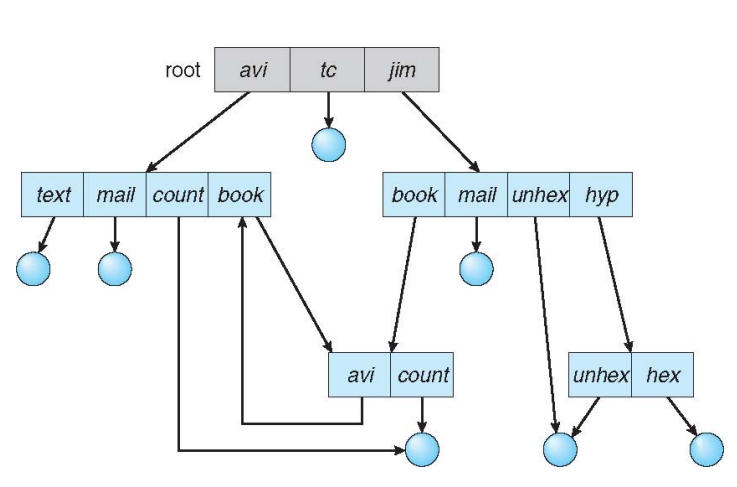
\includegraphics[width = 0.60\linewidth]{Images/29.png}
\end{center}
In questa struttura, vi è la possibilità di \textbf{hard links anche a directory a livelli superiori}, persino che contengono \textbf{ricorsivamente il link stesso}.
Per determinare se un file non è più referenziato, \textbf{un contatore al numero di riferimenti non basta più} ma occorre un autentico algoritmo di \textbf{garbage collection}.
Attraversare il file system in questo tipo di struttura diventa quindi ancora più complesso.
\subsection{Protezione}
Le informazioni devono essere preservate dai danni fisici (affidabilità) e dagli accessi impropri (protezione).
Un sistema multiutente permette un \textbf{accesso controllato ai file} di un certo utente da parte degli altri utenti.
Le operazioni controllabili sono:
\begin{itemize}
    \item Lettura
    \item Scrittura
    \item Esecuzione
    \item Aggiunta (scrittura in coda ad un file)
    \item Cancellazione
    \item Elencazione (elenco del contenuto di una directory)
\end{itemize}
\subsubsection{Liste di controllo degli accessi}
L'idea questo tipo di protezione è la seguente:
\begin{itemize}
    \item Ad ogni file/directory è associata una \textbf{lista di controllo degli accessi} (access control list, ACL)
    \item l'ACL specifica gli utenti \textbf{che possono accedere al file/directory}, con i relativi permessi di accesso
    \item Il file system controlla l'ACL prima di ogni accesso al file
\end{itemize}
Il \textbf{principale svantaggio} di questo approccio è che le ACL \textbf{possono diventare molto lunghe}.
Nei sistemi Unix-like, l'approccio usato è \textbf{raggruppare gli utenti in classi distinte}:
\begin{itemize}
    \item \textbf{Proprietario}: l'utente che possiede il file/directory
    \item \textbf{Gruppo}: il gruppo di utenti che condivide il file/directory
    \item \textbf{Pubblico}: tutti gli altri utenti
\end{itemize}
Facciamo un esempio:
\begin{table}[H]
    \centering
    \begin{tabular}{|c|c|ccc|}
    \hline
    Gruppo       & Bit di permesso (base 10) & \multicolumn{1}{c|}{r} & \multicolumn{1}{c|}{w} & x \\ \hline
    Proprietario & 7                         & 1                      & 1                      & 1 \\
    Gruppo       & 6                         & 1                      & 1                      & 0 \\
    Pubblico     & 4                         & 1                      & 0                      & 0 \\ \hline
    \end{tabular}
\end{table}
\noindent
Supponiamo di avere un file \textit{game}, di volergli assegnare un gruppo G e di volergli attribuire i permessi di cui sopra.
Allora procediamo come segue:
\begin{itemize}
    \item \textit{chgrp G game  \# cambia gruppo al file game}
    \item \textit{chmod 764 game  \# cambia i permessi al file game}
\end{itemize}
\subsection{Volumi e montaggio}
Un sistema operativo deve permettere di aggiungere e rimuovere dinamicamente unità di memorizzazione dati.
Un dispositivo di archiviazione può essere suddiviso in \textbf{partizioni}:
\begin{center}
    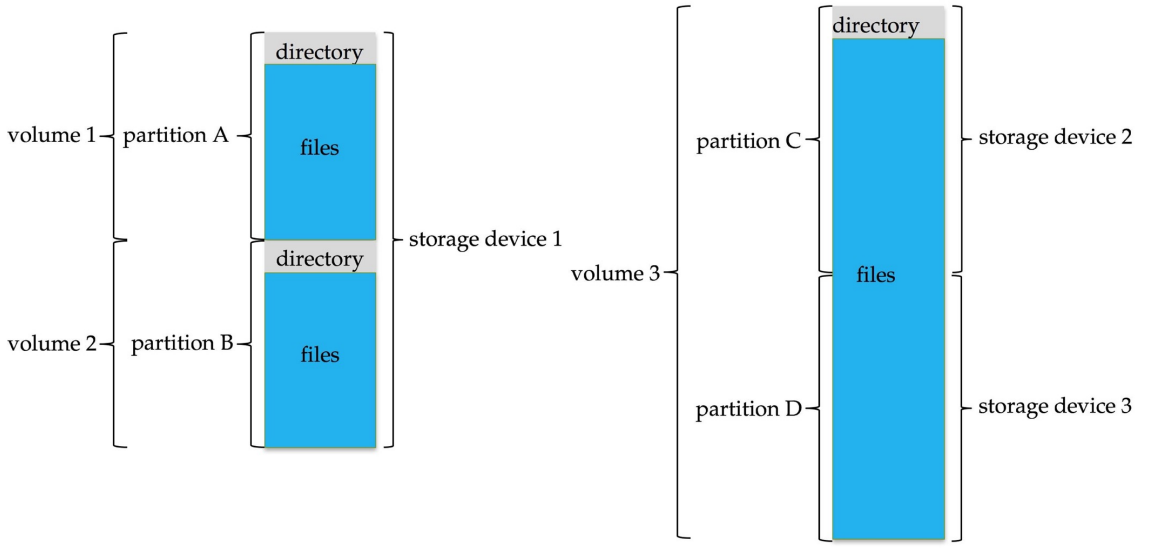
\includegraphics[width = 0.80\linewidth]{Images/30.png}
\end{center}
Un \textbf{volume} è una \textbf{zona di un dispositivo di archiviazione contenete un file system}.
Un volume, di solito, è contenuto in una partizione, su un solo dispositivo,
ma per alcuni filesystem particolari, un volume si può \textbf{estendere su più partizioni/dispositivi}.
Il sistema operativo deve permette di \textbf{montare e smontare} un volume all'interno dello spazio dei nomi del file system.
Di solito per montare un volume occorre fornire al sistema operativo:
\begin{itemize}
    \item L'identificazione del dispositivo/partizione dove risiede il volume
    \item Il punto di montaggio, ossia la \textbf{locazione nella struttura di file e directory alla quale "agganciare" il file system contenuto nel volume} (tipicamente una directory vuota)
\end{itemize}
Esistono diverse varianti di questo meccanismo:
\begin{itemize}
    \item \textbf{Punto di montaggio}: directory vuota oppure no
    \item \textbf{Montaggio}: automatico o manuale
    \item \textbf{Utilizzo di identificatori (lettere) di unità} anziché punti di montaggio
    \item \textbf{Montaggio ripetuto di uno stesso volume permesso} oppure no
\end{itemize}
\begin{center}
    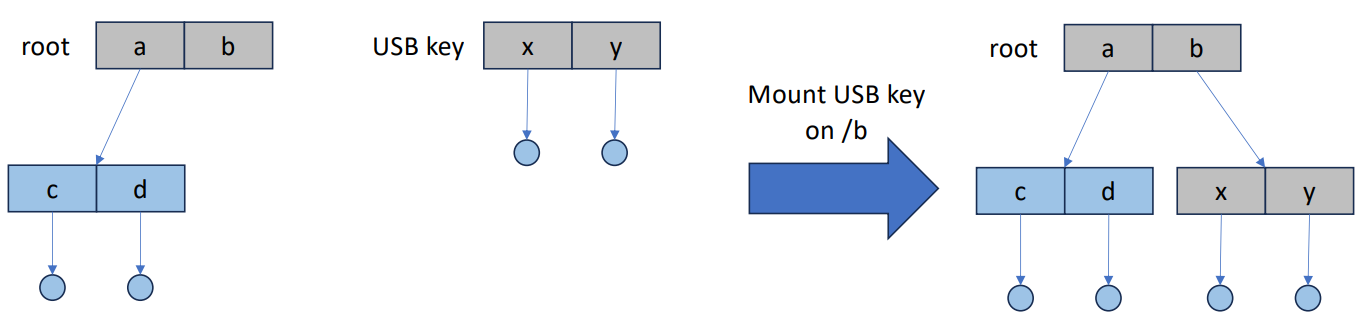
\includegraphics[width = 1\linewidth]{Images/31.png}
\end{center}
\subsection{API POSIX per operazioni sui file}
Per creare un file, possiamo utilizzare l'API \textit{creat}:
\begin{center}
    \textit{int creat(const char* path, mode\_t mode);}
\end{center}
Essa si comporta tuttavia come se fosse implementata nel seguente modo:
\begin{center}
    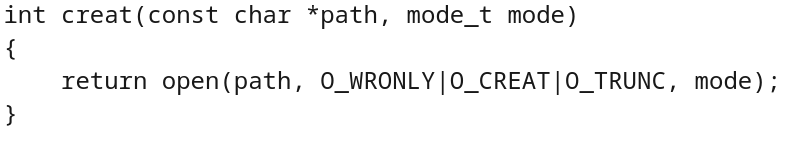
\includegraphics[width = 0.80\linewidth]{Images/32.png}
\end{center}
Quindi il parametro \textit{mode} dovrà assumere i valori delle flag presentate per \textit{open}. I valori
di ritorno della funzione saranno quindi quelli della funzione \textit{open}.
Per creare un file \textit{foot.txt} con diritti di lettura e scrittura per il proprietario, e di sola lettura per i membri
del gruppo e gli altri possiamo fare nel seguente modo:
\begin{center}
    \textit{int fd = creat("foo.txt", S\_IRUSR|S\_IWUSR|S\_IRGRP|S\_IROTH);}
\end{center}
oppure possiamo chiamare direttamente \textit{open}.
Per aprire un file, possiamo usare l'API \textit{open} (già presentata), mentre per leggere da un file
possiamo usare la funzione \textit{read} (già presentata).
Per scrivere su un file possiamo usare la funzione \textit{write} (già presentata), mentre per \textbf{riposizionarci all'interno di un file} possiamo usare
la funzione \textit{lseek}
\begin{center}
    \textit{off\_t lseek(int fildes, off\_t offset, int whence);}
\end{center}
La funzione riposizionerà il puntatore per il file aperto associato al file descriptor \textit{fildes} nel seguente modo:
\begin{itemize}
    \item Se \textit{whence} ha valore \textit{SEEK\_SET}, il puntatore sarà impostato al byte \textit{offset}
    \item Se \textit{whence} ha valore \textit{SEEK\_CUR}, il puntatore sarà impostato al byte corrispondente alla somma della posizione corrente e di \textit{offset}
    \item Se \textit{whence} ha valore \textit{SEEK\_END}, il puntatore sarà impostato alla fine del file più \textit{offset}
    \item Se \textit{whence} ha valore \textit{SEEK\_HOLE}, il puntatore sarà impostato alla prima posizione con un "buco" (regione del file senza dati) con grandezza maggiore o uguale a \textit{offset}, a meno che \textit{offset} non cada oltre l'ultimo byte non all'interno di un buco; in questo caso, il puntatore viene impostato all'ultimo byte del file (cioè, c'e sempre un buco implicito alla fine di ogni file)
    \item Se \textit{whence} ha valore \textit{SEEK\_DATA}, il puntatore sarà impostato alla più piccola posizione di un byte che NON è in un buco a distanza minima \textit{offset} dalla posizione corrente. Verrà dato errore se questo byte non esiste
\end{itemize}
Le flag appena presentate sono presenti nella libreria \textit{unistd.h}.
Un esempio del suo utilizzo è il seguente:
\begin{center}
    \textit{off\_t offset = lseek(fd, 10, SEEK\_CUR); // 10 bytes dopo la posizione corrente}
\end{center}
La funzione ritornerà l'offset risultante, misurato in byte dall'inizio del file, se ha successo, altrimenti -1.
Per chiudere un file utilizziamo l'API \textit{close} (già presentata), mentre per cancellarlo dal file system usiamo l'API \textit{unlink} (già presentata).
Per troncare un file invece fino ad una lunghezza $n$, possiamo usare la funzione \textit{truncate}:
\begin{center}
    \textit{int truncate(const char* path, off\_t length);}
\end{center}
La funzione quindi troncherà il file identificato dal path \textit{path} fino alla posizione \textit{length} (cioè imposta la sua lunghezza a \textit{length}).
I dati presenti dopo \textit{length} sono \textbf{scartati}. La funzione ritornerà 0 se ha successo, -1 altrimenti. Un esempio del suo uso può essere il seguente:
\begin{center}
    \textit{int ok = truncate("foo.txt", n); //tronca il file alla lunghezza n}
\end{center}
\subsubsection{API POSIX per i lock}
In POSIX, i lock sui file sono \textbf{consultivi}. Il lock su un file si può effettuare con l'operazione \textit{fcntl}, che è un API che permette di effettuare \textbf{diversi tipi di operazioni sui file}. La sua firma è:
\begin{center}
    \textit{int fcntl(int fildes, int cmd, ...);}
\end{center}
Essa ha parecchie funzionalità, quindi qui ci concentreremo solo su quelle necessarie per effettuare un lock.
Occorre specificare il tipo di lock utilizzando una \textbf{struct flock}. Se si vuole effettuare un lock su un file puntato da \textit{fildes}, l'argomento di \textit{cmd} dovrà essere
\textit{F\_SETLK}. Vediamo un esempio:
\begin{center}
    \textit{struct flock fl;} \\
    \textit{fl.l\_type = F\_RDLCK; // read lock} \\
    \textit{fl.l\_whence = SEEK\_CUR; // dalla posizione corrente...} \\
    \textit{fl.l\_start = 10; //...più 10 byte} \\
    \textit{fl.l\_len = 0; //fino alla fine del file} \\
    \textit{int ok = fcntl(fd, F\_SETLK, \textnormal{\&}fl); // se non riesce ad impostare un lock, fallisce}
\end{center}
\subsection{API POSIX per operazioni su directory}
Per creare una nuova directory, possiamo usare la funzione \textit{mkdir}
\begin{center}
    \textit{int mkdir(const char* path, mode\_t mode);}
\end{center}
Essa creerà una nuova directory con nome \textit{path}. Il parametro \textit{mode} indica i bit di permesso per la nuova directory.
Per esempio, creiamo una nuova directory, con diritti di lettura, scrittura e ricerca per il proprietario e di sola lettura per i membri del gruppo e gli altri nel seguente modo:
\begin{center}
    \textit{mkdir("/home/pietro/newdir", S\_IRWXU|S\_IRGRP|S\_IROTH);}
\end{center}
La funzione restituisce 0 se ha successo, -1 altrimenti. Come si può notare, possiamo anche usare le flag viste in precedenza, concatenare con un bitwise inclusive OR (|), per specificare
i permessi. Per eliminare una directory (solo se vuota) possiamo usare la funzione \textit{rmdir}:
\begin{center}
    \textit{int rmdir(const char* path);}
\end{center}
La funzione rimuoverà la directory specificata da \textit{path}. Ritorna 0 se ha successo, -1 altrimenti. Un esempio di un suo utilizzo può essere il seguente:
\begin{center}
    \textit{rmdir("/home/pietro/newdir");}
\end{center}
Possiamo aprire una directory tramite l'API \textit{opendir}:
\begin{center}
    \textit{DIR *opendir(const char *dirname);}
\end{center}
La funzione aprirà la directory specificata da \textit{dirname} (in particolare, apre un \textbf{directory stream}, che è una sequenza ordinata di tutte le voci in una directory). La funzione ritornerà un \textbf{puntatore ad una struttura di tipo DIR} (cioè un puntatore al directory stream)
se ha successo, altrimenti ritornerà un puntatore a null. Per leggere da una directory possiamo usare l'API \textit{readdir}:
\begin{center}
    \textit{struct dirent* readdir(DIR *dirp);}
\end{center}
La funzione ritornerà un puntatore ad una struttura \textit{dirent}, definita in \textit{dirent.h}, che rappresenta la voce nella directory alla posizione corrente nello stream specificato nell'argomento \textit{dirp}; dopodiche posizionerà
lo stream \textbf{alla prossima voce della directory}. Se la funzione incontra un errore oppure arriva alla fine della directory, ritornerà un puntatore a null.
Per cambiare il nome, o spostare, un file o una directory si può usare l'API \textit{link} in combinazione con l'API \textit{unlink}. Presentiamo prima la firma di \textit{link}:
\begin{center}
    \textit{int link(const char* path1, const char* path2);}
\end{center} 
La funzione creerà un nuovo \textbf{hard link} nel percorso \textit{path2} per il file 
identificato dal \textit{path1}. La funzione ritorna 0 se ha successo, -1 altrimenti.
Per ottenere l'effetto descritto sopra, possiamo fare come segue: supponiamo di voler spostare il file \textit{/foo/bar} nella directory \textit{/home/pietro}
e, allo stesso tempo, cambiare il suo nome in \textit{baz}:
\begin{center}
    \textit{int ok1 = link("/foo/bar", "/home/pietro/baz");} \\
    \textit{int ok2 = unlink("/foo/bar");}
\end{center}
Quando il link count di un file \textbf{arriva a zero}, il file \textbf{viene cancellato}.
Per creare un link simbolico, possiamo usare l'API \textit{symlink}:
\begin{center}
    \textit{int symlink(const char* path1, const char* path2);}
\end{center}
La funzione creerà un link simbolico chiamato \textit{path2} per il file con path \textit{path1}. Facciamo un esempio:
\begin{center}
    \textit{int ok = symlink("/home/pietro/baz", "/home/pietro/alias");}
\end{center}
I link simbolici non vengono aggiunti al link count.
\subsection{API POSIX per la protezione}
In POSIX, la protezione è basata su bit di lettura/scrittura/esecuzione per i gruppi proprietario/gruppo/pubblico.
Per cambiare il proprietario eil gruppo di un file possiamo usare la funzione \textit{chown}:
\begin{center}
    \textit{int chown(const char *path, uid\_t owner, gid\_t group);}
\end{center}
La funzione imposterà per il file in \textit{path} \textit{owner} come nuovo proprietario del file e \textit{group} come nuovo gruppo di appartenenza.
La funzione ritorna 0 se ha successo, -1 altrimenti.
Facciamo un esempio:
\begin{center}
    \textit{uid\_t owner = ...; // Un nuovo proprietario} \\
    \textit{gid\_t group = ...; // Un nuovo gruppo di appartenenza} \\
    \textit{int ok = chown("/home/pietro/baz, owner, group);}
\end{center}
Per cambiare i diritti di lettura/scrittura/esecuzione, possiamo usare la funzione \textit{chmod}:
\begin{center}
    \textit{int chmod(const char* path, mode\_t mode);}
\end{center}
La funzione imposterà i nuovi bit di permesso per il file in \textit{path} a \textit{mode}, la quale può essere
descritta con le flag viste fino ad ora per \textit{mode}, concatenate con un bitwise inclusive OR. Facciamo un esempio:
\begin{center}
    \textit{int ok = chmod("/home/pietro/baz", S\_IRUSR | S\_IRGRP);}
\end{center}
la funzione ritornerà 0 se ha successo, -1 altrimenti.
\section{Interfaccia e struttura del kernel}
Un'implementazione delle API attraverso chiamate di sistema segue il seguente schema:
\begin{center}
    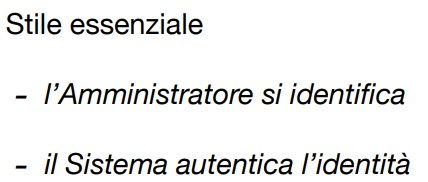
\includegraphics[width = 0.80\linewidth]{Images/33.png}
\end{center}
ciò permette al sistema operativo di proteggere se stesso dai programmi in esecuzione.
La CPU può funzionare in \textbf{modalità utente} (user mode) o in \textbf{modalità di sistema} (kernel mode) impostano un opportuno \textbf{bit di modalità}.
Alcune istruzione del processore sono quindi \textbf{privilegiate}, ossia sono eseguibili solamente in kernel mode: in particolare, in user mode la CPU \textbf{non può accedere alla memoria del kernel}.
Una chiamata di sistema non è quindi semplice da implementare come una normale chiamate a funzione, poiché occorre \textbf{effettuare una transizione da modalità utente a modalità di sistema}:
\begin{enumerate}
    \item Vengono prima \textbf{preparati i parametri necessari}
    \begin{itemize}
        \item Un numero che identifica quale chiamata di sistema va effettuata...
        \item ...più tutti i parametri necessari alla specifica chiamata di sistema
    \end{itemize}
    \item Quindi, viene invocata un'opportuna \textbf{istruzione macchina} che genera un'eccezione software; essa fa passare la CPU in kernel mode e trasferisce il controllo ad una \textbf{subroutine} ad un determinato indirizzo di memoria
    \item La subroutine, chiamata \textbf{system call interface}, legge il numero identificativo della chiamata di sistema, effettua un \textbf{lookup da una tabella interna dell'indirizzo della routine che effettivamente implementa la chiamata di sistema}, e salta a tale indirizzo
    \item La routine invocata legge i parametri ed esegue la funzionalità richiesta
    \item Al ritorno, il processore passa di nuovo in user mode
\end{enumerate}
\begin{center}
    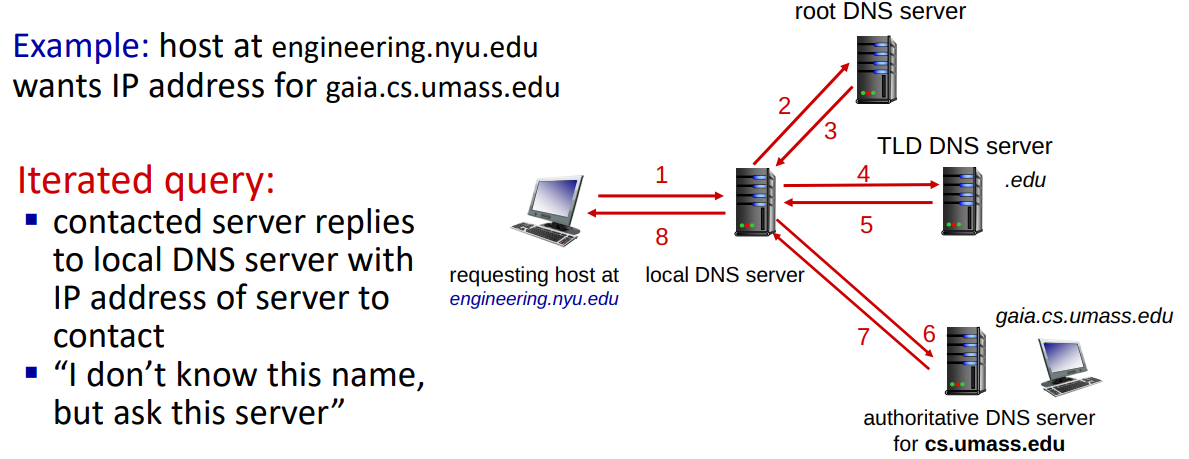
\includegraphics[width = 1\linewidth]{Images/34.png}
\end{center}
Come avviene quindi il passaggio dei parametri alle chiamate di sistema? Dal momento che l'invocazione delle chiamate di sistema passa per un'eccezione software,
il passaggio di parametri è più complesso rispetto a quello di una normale chiamata di procedura. Vi sono diversi modi:
\begin{itemize}
    \item \textbf{Metodo più semplice}: passare i parametri nei registri del processore
    \begin{itemize}
        \item \textbf{Vantaggio}: rapido
        \item \textbf{Svantaggio}: utile solo per pochi parametri i cui tipi di dati hanno dimensione limitata
    \end{itemize}
    \item \textbf{Altro metodo:} passo in uno dei registri un indirizzo di memoria ad un blocco nel quale sono memorizzati i parametri
    \begin{itemize}
        \item Utilizzato da Linux, insieme al primo metodo
    \end{itemize}
    \item \textbf{Altro metodo}: faccio push dei parametri sullo stack
    \begin{itemize}
        \item \textbf{Vantaggi}: flessibile, simile ad una normale chiamata di procedura
        \item \textbf{Svantaggi}: lento e macchinoso
    \end{itemize}
\end{itemize}
È necessario notare che \textbf{ogni thread ha di solito due stack}:
\begin{itemize}
    \item Quello che viene utilizzato dal programma in user mode
    \item Quello che viene utilizzato quando il thread \textbf{passa in kernel mode}
\end{itemize}
Una chiamata di sistema, come prima cosa, \textbf{imposta lo stack del thread corrente allo stack di sistema} e, al termine della chiamata di sistema, ripristina lo stack a quello utente.
Per quale motivo? \textbf{Per sicurezza}: dal momento che il processo potrebbe modificare a suo piacimento il registro stack pointer (che non è privilegiato), allora \textbf{non è possibile fidarsi che questo punti ad uno stack "sano"}:
pertanto, in kernel mode, occorre usare uno stack sicuramente corretto.
\subsection{Uso delle librerie dinamiche per le API}
Si vuole far si che, anche se il sistema operativo viene aggiornato, non vi sia bisogno di ricompilare/linkare le applicazioni qualora siano cambiate le chiamate di sistema, o l'implementazione delle API,
\textbf{purché l'interfaccia delle API resti la stessa}.
Un vantaggio si ha realizzando le API e le librerie standard del linguaggio come \textbf{librerie dinamiche}. Infatti, se queste sono modificate (nell'implementazione, non nell'interfaccia), non occorre
ricompilare tutti gli eseguibili per aggiornali alla nuova versione delle librerie.
Occorre però un'ulteriore accortezza: oltre all'API \textbf{non deve cambiare l'Application Binary Interface (ABI)}.
L'ABI è \textbf{l'insieme delle convenzioni attraverso le quali il codice binario dell'applicazione si interfaccia con il codice binario della libreria dinamica delle API}:
\begin{itemize}
    \item Come si chiama internamente alla libreria la funzione da invocare? (\textbf{name mangling})
    \item In che ordine i parametri vengono messi sullo stack delle chiamate?
    \item Come sono strutturati i tipi di dati? C'è padding? Qual è l'endianess? (Cioè, qual'è l'ordine da seguire per interpretare i byte) 
\end{itemize}
\subsection{La scarsa portabilità degli eseguibili binari}
Come facciamo ada vere applicazioni \textbf{portabili su diversi sistemi di elaborazione?}
Ci sono tre possibili approcci:
\begin{itemize}
    \item Scrivere l'applicazione in un linguaggio con un \textbf{interprete portatile} (es. Python, Ruby): in tal caso, \textbf{l'eseguibile è il sorgente}
    \item Scrivere l'applicazione in un linguaggio con un \textbf{ambiente runtime portatile} (es.Java, .NET): in tal caso, \textbf{l'eseguibile è il bytecode}
    \item Scrivere l'applicazione utilizzando un \textbf{linguaggio con un compilatore portatile ed API standardizzate}: l'eseguibile è \textbf{file binario compilato e linkato}
\end{itemize}
Nei primi due casi, l'eseguibile è normalmente \textbf{uno solo per tutte le architetture}.
Nel terzo caso invece, occorre, di norma, generare un eseguibile \textbf{distinto} a variazioni anche minime del sistema di elaborazione (spesso anche solo al variare della versione del sistema operativo).
Come mai?
\begin{itemize}
    \item Una prima banale ragione può essere la \textbf{differenza nell'architettura hardware}: ad esempio, un file binario prodotto per CPU ARM non può essere interpretato da un sistema di elaborazione con CPU x86-64, dal momento che le istruzioni macchina delle due CPU differiscono
    \item A parità di architettura hardware, \textbf{sistemi operativi diversi possono supportare API diverse}: ad esempio, Windows supporta le API Win32 e Win64 e non le API POSIX, supportate da Linux e MacOS
    \item A parità di architettura e API, \textbf{sistemi diversi possono supportare diversi formati per i file binari}: ad esempio, Linux riconosce il formato ELF, mentre macOS riconosce il formato MachO
    \item A parità di architettura, formato ed API, può esservi una \textbf{differenza nelle chiamate di sistema che le implementano} (se la libreria API è \textbf{collegata staticamente})
    \item A parità di architettura, formato ed API, anche se la libreria API è collegata dinamicamente (o le chiamate di sistema sono le stesse), \textbf{può esservi una differenza nell'ABI}
    \item Solo quanto tutti questi fattori sono identici, un file binario è portabile da un sistema di elaborazione ad un'altro
\end{itemize} 
\subsection{Struttura del Kernel}
Il kernel è strutturato in \textbf{sottosistemi}, basati sulle categorie dei servizi offerti dal kernel stesso (e quindi sulle categorie delle chiamate di sistema).
I principali sono:
\begin{itemize}
    \item Gestione dei processi e dei thread
    \item Comunicazione tra processi e sincronizzazione
    \item Gestione della memoria
    \item Gestione dell'I/O
    \item File System
\end{itemize}
Il kernel di un sistema operativo \textbf{general-purpose} è un programma
\begin{itemize}
    \item Di \textbf{dimensioni elevate e complesso}
    \item Che deve operare \textbf{molto rapidamente} per non sottrarre tempo di elaborazione ai programmi applicativi
    \item Un cui malfunzionamento può provocare il crash dell'intero sistema di elaborazione
\end{itemize}
Si pone quindi il problema di come progettarlo in maniera da garantire \textbf{rapidità e correttezza} nonostante dimensioni e complessità.
Alcune possibilità di struttura sono:
\begin{itemize}
    \item Struttura monolitica
    \item Struttura a strati
    \item Struttura a microkernel
    \item Struttura a moduli
    \item Struttura ibrida
\end{itemize}
\subsubsection{Struttura monolitica}
Il sistema operativo UNIX originale aveva una struttura monolitica, dove il kernel è un \textbf{singolo file binario statico}.
Il kernel forniva un elevato numero di funzionalità:
\begin{itemize}
    \item Scheduling della CPU
    \item File system
    \item Gestione della memoria, swapping, memoria virtuale
    \item Device drivers
    \item ...
\end{itemize}
I \textbf{vantaggi} di questa struttura sono \textbf{le sue elevati prestazioni}.
Tuttavia, essa soffre di un numero di \textbf{svantaggi}:
\begin{itemize}
    \item Complessità 
    \item Fragilità ai bug
    \item Necessità di \textbf{ricompilare il kernel} (e riavviare il sistema) se bisogna aggiungere una funzionalità, ad esempio il driver di una nuova periferica
\end{itemize}
\subsubsection{Struttura a strati}
Negli approcci stratificati, il sistema operativo è diviso in un \textbf{insieme di livelli, o strati}.
Lo strato più basso \textbf{interagisce con l'hardware}, lo strato n-esimo interagisce solo con lo strato $n-1$ esimo.
L'approccio offre \textbf{tre vantaggi}:
\begin{itemize}
    \item Ogni strato può essere progettato e implementato \textbf{indipendentemente dagli altri strati}
    \item È possibiel verifciare la \textbf{correttezza degli strati indipendentemente da quella degli altri strati}
    \item Ogni strato \textbf{nscone le funzionalità degli strati sottostanti} e presenta allo strato soprastante \textbf{una macchina dalle caratteristiche più astratte}
\end{itemize}
In realtà, pochi sistemti operativi usano questo approccio in maniera pura:
\begin{itemize}
    \item È difficile \textbf{definire esattamente quali funzionalità devono avere uno strato}
    \item Ogni strato introduce \textbf{un overhead} che peggiore le prestazioni
\end{itemize}
È comunque conveniente \textbf{strutturare alcune parti del sistema operativo a strati} (es. File System o stack di rete).
\subsubsection{Struttura a microkernel}
Il princiaple problema dei kernel monolitici è la loroc complessità e, di conseguenza, la loro fragilità e inaffidabilità.
La struttua a microkernel sposta \textbf{quanti più servizi possibile fuori dal kernel in programmi di sistema}, mantenendo nel kernel l'insieme
\textbf{minimo} di servizi indinspensabili per implementare gli altri.
Il kernel è definito microkernel \textbf{dal moemnto che ha dimensioni molto ridotte}.
L'approccio è stato proposto negli anni '80 con il sistema operativo Mach.
Un microkernel offre \textbf{pochi servizi}, di solito
\begin{itemize}
    \item Lo \textbf{scheduling dei processi}
    \item (Una parte della) \textbf{gestione della memoria}
    \item La \textbf{comunicazione tra processi}
\end{itemize}
Gli altri servizi (es. filesystem e device drivers) vengono implementati \textbf{a livello utente}.
Per chiedere un servizio, un programma \textbf{comunica con il programam di sistema che lo implementa attraverso le primitive di comunicazione offerte dal microkernel}.
\begin{center}
    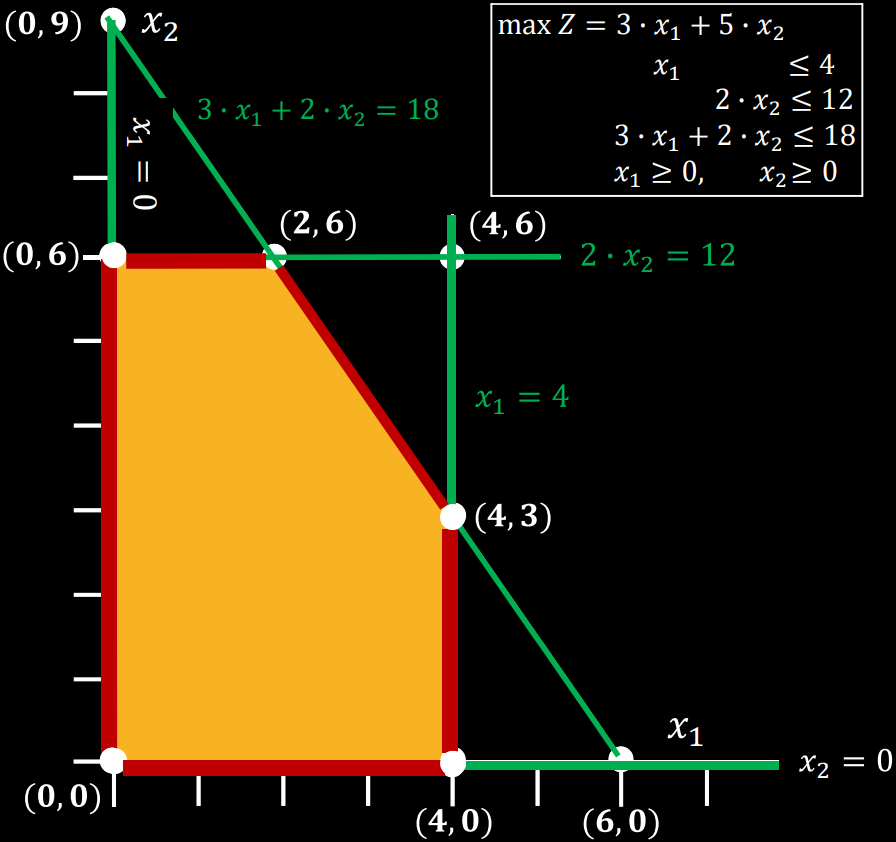
\includegraphics[width = 0.80\linewidth]{Images/35.png}
\end{center}
Vediamo i \textbf{vantaggi} di questa architettura:
\begin{itemize}
    \item Facilità di \textbf{estensione del sistema operativo}: posso aggiungere un nuovo servizio senza dover modificare il kernel
    \item \textbf{Maggiore affidabilità}: se un servizio va in crash, mon manda in crash il kernel; un kernel piccolo può essere quindi reso più affidabile con meno sforzo
\end{itemize}
vediamome quindi gli svantaggi:
\begin{itemize}
    \item \textbf{Overhead}: una tipica richiesta di servizio deve \textbf{transitare dal processo richiedente al microkernel, al processo di sistema destinatario e viceversa}, con molti passaggi tra user e kernel mode, comunicazioni, context switching ecc...
\end{itemize}
I sistemi a microkernel puri vegnono usati nelle applicazioni che \textbf{richiedono elevata affidabilità} (QNX neutrino, L4se). Altri sistemi, inizalmente a microkernel, si sono evoluti in \textbf{sistemi ibridi} (es. Windows NT, Darwin - kernel di macOS e iOS).
\subsubsection{Struttura a moduli}
In questa struttura, il kernel è \textbf{strutturato in componenti dinamicamente caricabili} (moduli), che parlano tra di loro \textbf{attraverso interfacce}.
Quando il kernel ha bisogno di offrire un certo servizio, carica \textbf{dinamicamente} il modulo che lo implementa; quando il servizio non è più necessario, il kernel può scaricare il modulo.
Questo approccio ha alcune \textbf{caratteristiche di quelli a strati e a microkernel}, ma i moduli \textbf{eseguono direttamente in kernel mode} e quindi con minore overhead (ma \textbf{anche con minore isolamento tra di loro}).
\subsubsection{Sistemi ibridi}
In pratica, pochi sistemi operativi adottano una struttura "pura": quasi tutti \textbf{combinano i diversi approcci allo scopo di sistemi operativi indirizzati alle prestazioni, sicurezza, usabilità, ...}
Per esempio, Linux e Solaris sono \textbf{monolitici per avere prestazioni elevate}, ma supportano anche i \textbf{moduli del kernel} per poter caricare e scaricare dinamicamente funzionalità.
Altro esempio è Windows, il quale kernel inzialmente aveva una \textbf{struttura a microkernel}, ma successivamente diversi servizi sono stati riportati nel kernel per migliorare le prestazioni.
Ora è essenzialmente \textbf{monolitico}, pur conservando alcune caratteristiche della precedente architettura a microkernel. Inoltre, supporta i \textbf{moduli del kernel}.
\subsection{Politiche e meccanismi}
Quando discutiamo come è realizzato il kernel, è importante distinguere tra \textbf{politiche} e \textbf{meccanismi}.
\begin{itemize}
    \item Una \textbf{politica} dice \textbf{QUANDO} una certa operazione viene effettuata: ad esempio, sotto che condizioni il kernel decide che è il momento di sospendere l'esecuzione di un programma per far riprendere l'esecuzione di un altro? (Preemption)
    \item Un \textbf{meccanismo} spiega \textbf{COME} una certa operazione è effettuata: ad esempio, come fa il kernel a sospsendere l'esecuzione di un programma in maniera che successivamente possa riprnedere? Come fa a ripristinare l'esecuzione di un prrogramma precedentemente sospeso?
\end{itemize}
Le politiche \textbf{impattano profondamente} sulle caratteristiche percepite dal sistema di elaborazione, i meccanismi no.
I meccansimi sono quindi più \textbf{stabili} delle politiche, che spesso cambiano in funzione delle caratteristiche perceptie che vogliamo che il sistema di elaborazione abbia.
Avere politiche configurabili è utile per combattere la \textbf{maledizione della generalità}.
\section{Processi e Thread: la struttura}
I sistemi operativi hanno due obiettivi:
\begin{itemize}
    \item \textbf{Efficienza}: mantenere impeganta la (o le) CPU il maggior tempo possibile nell'esecuzione dei programmi (se ci sono programmi da eseuire)
    \item \textbf{Reattività}: Dare l'illusione che ogni processo progredisca continuamente nella propria esecuzione, come se avesse una CPU dedicata; questo è particolarmente importante per i \textbf{programmi interattivi}, che devono reagire in tempi accettabili quando ricevono un input utente.
\end{itemize}
Le due tecniche adottate nei sistemi operativi per ottenere questi due obbiettivi sono la \textbf{multiprogrammazione} e il \textbf{multitasking} (o \textbf{time-sharing}):
\begin{itemize}
    \item \textbf{Obbiettivo della multiprogrammazione}: impredire che un programma non è in condizione di proseguire l'esecuzione mantenga la CPU
    \item \textbf{Obbiettivo del multitasking}: Far si che un programma interattivo possa reagire agli input utente in un tempo accettabile
\end{itemize}
Bisogna notare che la multiprogrammazione non è una tecnica rilevante per i sistemi \textbf{puramenti batch} (cioè che non richiedono un input utente).
L'obbiettivo della multiprogrammazione è massimizzare l'utilizzo della CPU. Gli \textbf{algoritmi di scheduling} sfruttano il fatto che, di norma, l'esecuzione di un processo è una sequenza di:
\begin{itemize}
    \item \textbf{Burst della CPU}: seqeunza di operazioni di CPU
    \item \textbf{Burst dell'I/O}: Attesa completamento di un'operazione di I/O
\end{itemize}
\begin{center}
    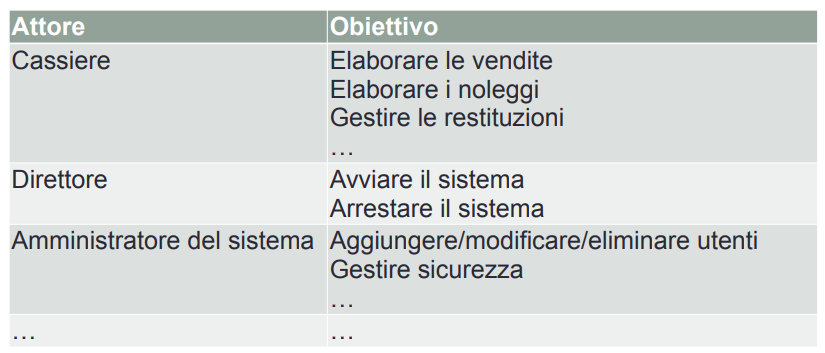
\includegraphics[width = 0.28\linewidth]{Images/36.png}
\end{center}
Diventa quindi necessario \textbf{gaurdare alla distribuzione delle durate dei burst della CPU}.
In un programma, quindi, si potrebbe avere
\begin{itemize}
    \item \textbf{Prevalenza di burst I/O} (I/O Bound)
    \begin{itemize}
        \item Elevato numero di burst CPU brevi
        \item Ridotto numero di burst CPU lunghi
        \item Tipico dei \textbf{programmi interattivi}
    \end{itemize}
    \item \textbf{Programma con prevalenza di CPU} (CPU Bound)
    \begin{itemize}
        \item Elevato numero di burst CPU lunghi
        \item Ridotto numero di burst CPU brevi
        \item Tipico dei programmi batch
    \end{itemize}
\end{itemize}
In entrambi i casi, la curva della distribuzione ha la forma riportata sotto, ma:
\begin{itemize}
    \item \textbf{I/O Bound}: il massimo sta più a sinistra
    \item \textbf{CPU Bound}: il massimo sta più a destra
\end{itemize} 
\begin{center}
    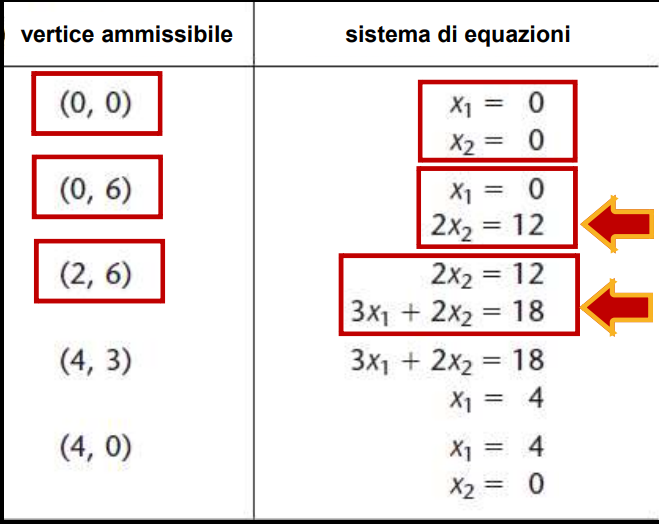
\includegraphics[width = 0.58\linewidth]{Images/37.png}
\end{center}
\subsection{Multiprogrammazione}
Il sistema operativo mantiene in memoria le immagini dei processi da eseguire.
Quando una CPU non è impeganta ad eseguire un processo, il sistema operativo \textbf{seleziona un processo non in esecuzione e gli assegna la CPU}.
Quando un processo non può proseguire l'esecuzione (ad es. perché deve attendere il termine dell'input di dati che gli servono per proseguire), la sua CPU
\textbf{viene assegnata ad un altro processo non in esecuzione}.
Come risultato, se i processo sono più delle CPU, queste saranno impegante nell'esecuzione di qualche processo per la maggior parte del tempo.
\subsubsection{Multiprogrammazione e memoria}
La multiprogrammazione richiede che tutte le immagini di tutti i processi siano in memoria perché questi possano essere eseguibili.
Se i processi sono troppi e non possono essere contenuti tutti in memoria, si adotta una tecnica che prende il nome di \textbf{swapping}, la quale viene utilizzata
per spostare le immagini dei processi dentro/fuori dalla memoria.
Se l'immagine di un processo è \textbf{troppo grande}, la \textbf{memoria virtuale} è un'ulteriore tecnica che permette di eseguire un processo la cui immagine \textbf{non è completamente in memoria}.
Queste tecniche aumentano il numero di processo che possono essere eseguiti in multiprogrammazione, ossia aumentano il \textbf{grado di multiprogrammazione}.
Approfondiremo più avanti tutti questi aspetti.
\subsection{Multitasking}
Il multitasking è \textbf{un'estensione della multiprogrammazione} per i sistemi interattivi.
La CPU viene "sottratta" periodicamente al programma in esecuzione ed assegnata ad un altro programma.
In questo modo, tutti i programmio \textbf{progrediscono in maniera continuativa nella propria esecuzione}, anziché solo
nei momenti in cui il programma che detiene la CPU si mette in attesa.
Questo fa si che i programmi batch, che hanno burst CPU lunghi pochi burst I/O, non monopolizzino la CPU a discapito dei programmi interattivi.
\subsection{Implementazione di un processo}
L'implementazione di un processo avviene tramite una struttura dati che prende il nome di \textbf{Process Control Block} (PCB) (detto anche \textbf{Task Control Block}).
Esso è la struttura dati del kernel che \textbf{contiene tutte le informazioni relative ad un processo}:
\begin{center}
    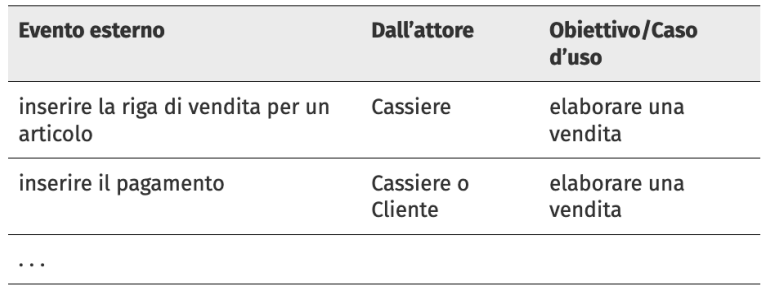
\includegraphics[width = 0.23\linewidth]{Images/38.png}
\end{center}
\begin{itemize}
    \item \textbf{Process state}: lo stato del processo (ready, running, ...)
    \item \textbf{Process number} (o PID): Identifica univocamente il processo
    \item \textbf{Program Counter}: contenuto del registro \textbf{program counter} ("istruzione successiva")
    \item \textbf{Registers}: Contenuto dei registri del processore
    \item \textbf{Informazioni relative alla gestione della memoria}: memoria \textbf{allocata} al processo
    \item \textbf{Informazioni sull'I/O}: dispositivi assegnati al processo, elenco di file aperti, ... 
    \item \textbf{Informazioni di scheduling}: Priorità, puntatori a code di scheduling, ... 
    \item \textbf{Informazioni di accounting}: CPU utilizzata, tempo trascorso, ... 
\end{itemize}
Durante l'esecuzione, un processo cambia più volte \textbf{stato}. Gli stati possibili di un processo sono:
\begin{itemize}
    \item \textbf{New}: il processo è creato, ma non ancora ammesso all'esecuzione
    \item \textbf{Ready}: Il processo può essere eseguito (è in attesa che gli sia assegnata una CPU)
    \item \textbf{Running}: Le sue istruzioni vengono eseguite da qualche CPU
    \item \textbf{Waiting}: Il processo non può essere eseguito perché è in attesa che si verifichi qualche evento (ad es. il completamente di un'operazione di I/O)
    \item \textbf{Terminated}: Il processo ha terminato l'esecuzione
\end{itemize}
\begin{center}
    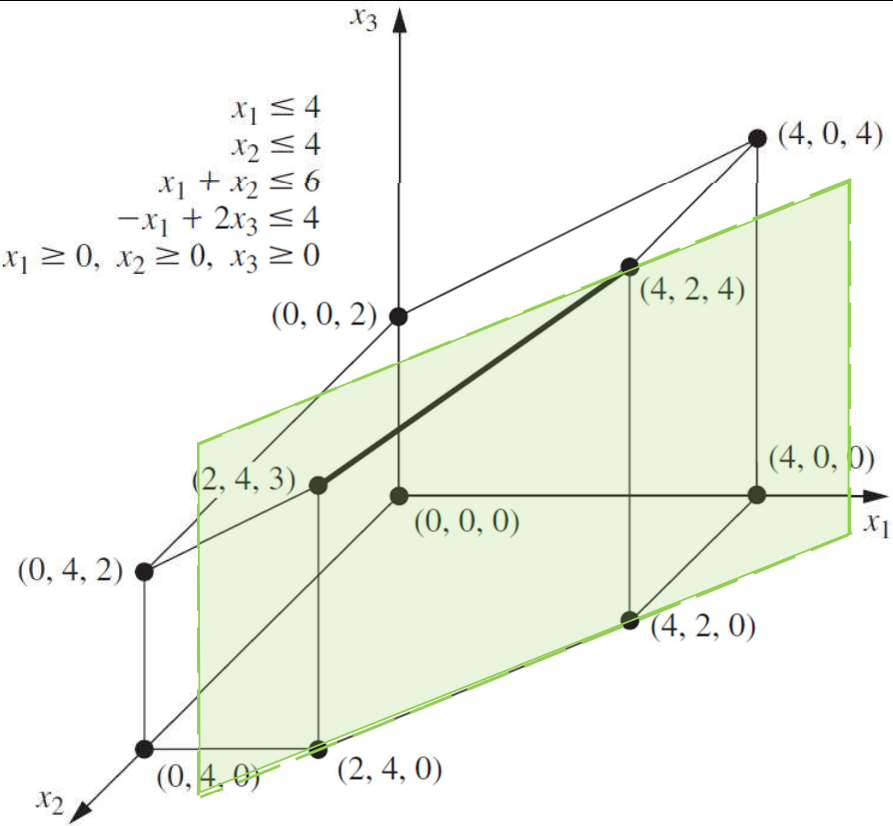
\includegraphics[width = 0.73\linewidth]{Images/39.png}
\end{center}
\subsection{CPU scheduling}
Lo \textbf{scheduler della CPU}, o \textbf{scheduler a breve termine}, sceglie il prossimo processo da eseguire tra quelli \textbf{in stato ready} ed alloca un core libero ad esso.
Mantiene quindi \textbf{diverse code di processi}:
\begin{itemize}
    \item \textbf{Ready queue}: processi residenti in memoria e in stato ready
    \item \textbf{Wait queue}: code per i processi che sono residenti in memoria e in stato di wait; una coda diversa \textbf{per ciascun diverso tipo di evento di attesa}
\end{itemize}
Durante la loro vita, i processi (i loro PCB) \textbf{migrano da una coda all'altra a seconda dello stato del processo stesso}.
\begin{center}
    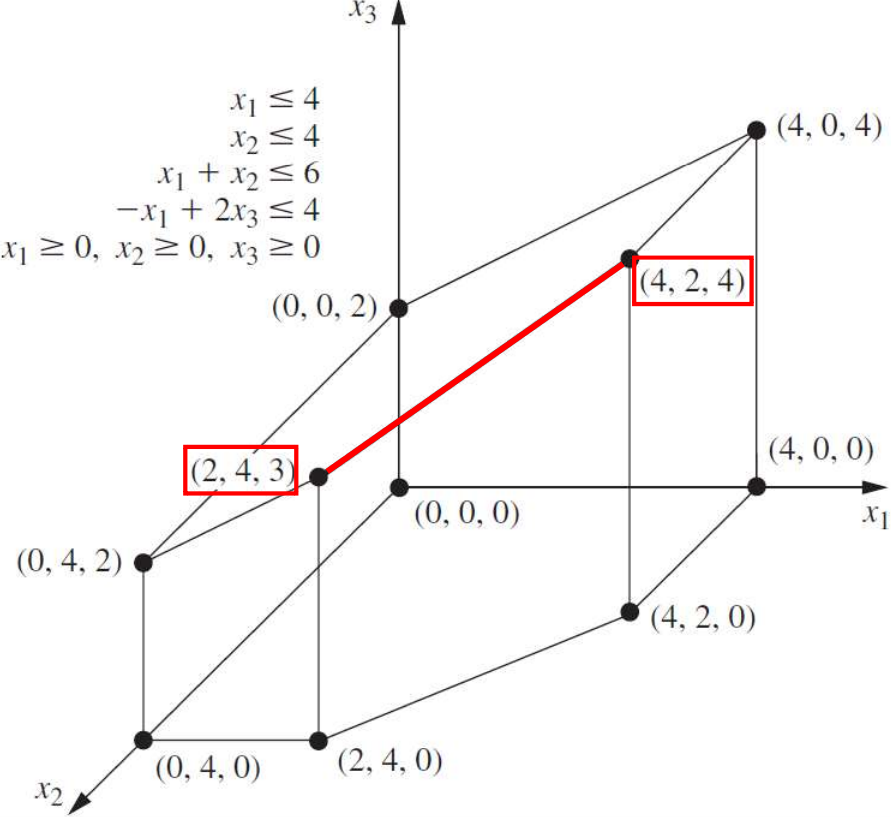
\includegraphics[width = 0.60\linewidth]{Images/40.png}
\end{center}
Lo scheduler della CPU ha il compito di \textbf{decidere a quale processo, tra quelli nella ready queue, assegnare un core libero}.
Tali \textbf{decisioni di scheduling} possono essere effettuate in diversi momenti, corrispondenti a \textbf{cambi di stato dei processi}:
\begin{enumerate}
    \item Quando un processo passa da stato running a stato waiting
    \item Quando un processo passa da stato running a stato ready
    \item Quando un processo passa da stato waiting a stato ready
    \item Quando un processo termina
\end{enumerate}
Se il riassegnamento viene fatto solo nelle situazioni 1 e 4, lo \textbf{schema di scheduling} è detto \textbf{senza prelazione} (\textbf{non-preemptive}) o \textbf{cooperativo}, dal momento che un core viene liberato
solamente quando un processo \textbf{volontariamente rinuncia ad esso}.
Altrimenti, è detto \textbf{con prelazione} (\textbf{preemptive}), dal momento che un core può essere liberato perché un core viene \textbf{forzatamente} sottrato dal kernel ad un processo che lo sta usando.
Lo schema di scheduling preemptive \textbf{è più complicato da implementare}:
\begin{itemize}
    \item Che succede se due processi condividono i dati?
    \item Che succede se un processo sta eseguendo in kernel mode? (System Call o Interrupt Request)
\end{itemize}
Quando il controllo della CPU deve passare da un processo ad un altro processo scelto dallo scheduler a breve termine, avviene una \textbf{commutazione di contesto} (\textbf{context switch}).
La commutazione di contesto viene effettuata dal \textbf{dispatcher}, che:
\begin{itemize}
    \item \textbf{Salva il contesto} (stato, registri) del processo da interrompere nel suo PCB
    \item \textbf{Carica il contesto} del processo da eseguire dal suo PCB
    \item \textbf{Passa in user mode}
    \item \textbf{Salta} nel punto corretto del programma del processo selezionato (ossia, dove era stato \textbf{precedentemente interrotto})
\end{itemize}
\begin{center}
    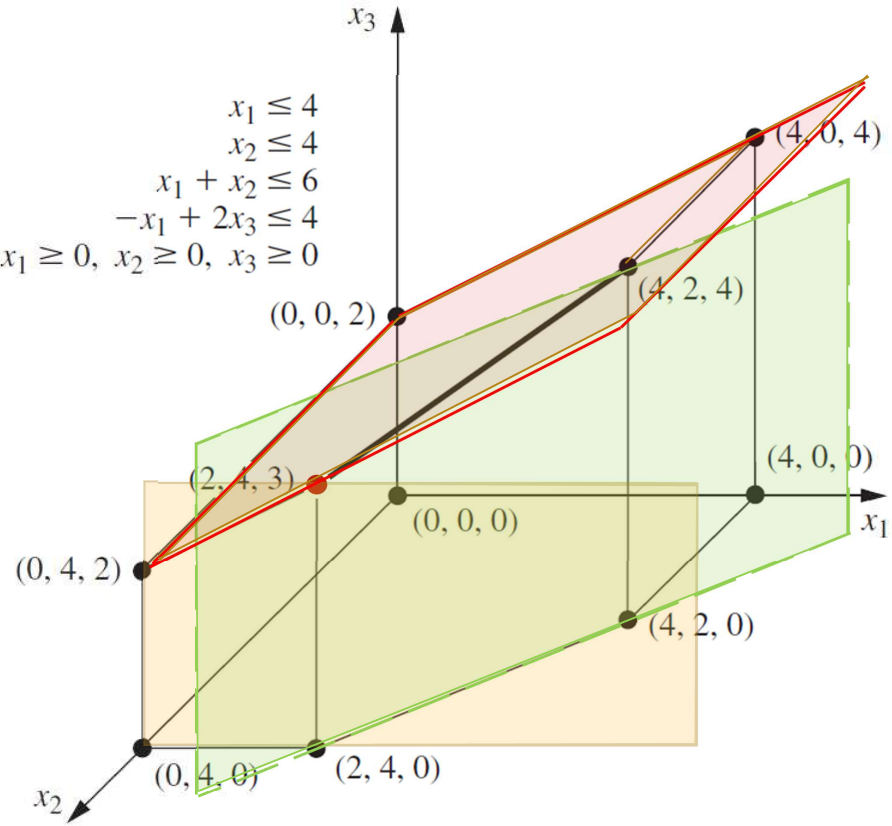
\includegraphics[width = 0.60\linewidth]{Images/41.png}
\end{center}
Notare che il dispatcher implementa un \textbf{tipico meccanismo}, mentre lo scheduler \textbf{implementa una tipica politica}.
La \textbf{latenza di dispatch} è il tempo impiegato dal dispatcher per fermare un processo ed avviarne un altro. La latenza di dispatch
è \textbf{puro overhead}: non viene eseguito alcun lavoro utile (definito come l'esecuzione di un programma utente).
Più è complesso il sistema operativo, più è complesso il PCB (il contesto), \textbf{maggiore è la latenza di dispatch}.
Alcuni processori offrono supporto speciale per \textbf{minimizzare la latenza di dispatch} (es. banchi di registri multipli).
\subsection{Implementazione dei thread}
Vi sono due tipi di thread:
\begin{itemize}
    \item \textbf{Thread a livello utente}: i thread disponibili nello spazio utente dei processi; sono quelli offerti dalle librerie di thread ai processi
    \item \textbf{Thread a livello kernel}: i thread implementati nativamente dal kernel; sono utilizzati per strutturare il kernel stesso \textbf{in maniera concorrente}
\end{itemize}
I thread a livello del kernel vengono utilizzati dalle librerie di thread per \textbf{implementare i thread a livello utente di un certo processo}.
A tale scopo, possono essere adottate diverse strategie (modelli di \textbf{multithreading}):
\begin{itemize}
    \item \textbf{Molti-a-uno}: I thread a livello utente di un certo processo sono implementati su un solo thread a livello del kernel
    \begin{itemize}
        \item \textbf{Vantaggio}: usabile su ogni sistema operativo (unica soluzione possibile se il sitema operativo non è multithreaded)
        \item \textbf{Svantaggio}: Se un thread utente fa una chiamata di sistema bloccante blocca tutti i thread utente dello stesso processo
        \item \textbf{Altro svantaggio}: non sfrutta la presenza di più core
        \item Poco usata in pratica
        \item Esempi: Solaris Green Threads e GNU Portable Threads
    \end{itemize}
    \begin{center}
        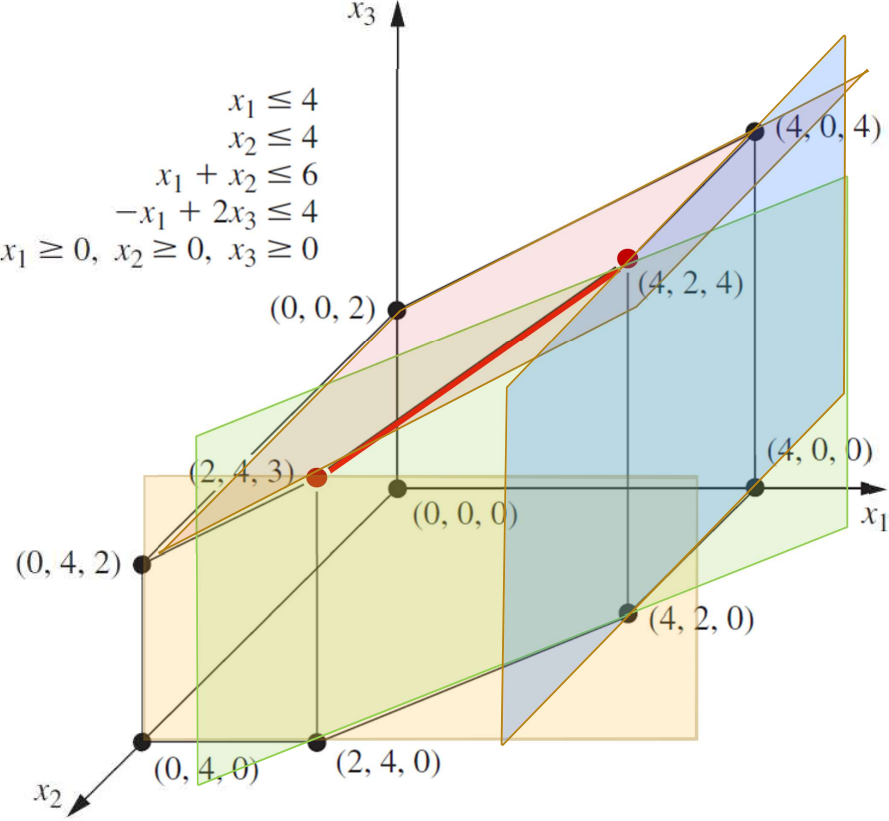
\includegraphics[width = 0.40\linewidth]{Images/42.png}
    \end{center}
    \item \textbf{Uno-a-uno}: Ogni thread a livello utente è implementato su un singolo, distinto thread a livello del kernel
    \begin{itemize}
        \item \textbf{Vantaggio}: permette un maggior grado di concorrenza
        \item \textbf{Vantaggio}: permette di sfruttare il parallelismo nei sistemi multicore
        \item \textbf{Svantaggio}: minore performance rispetto al modello molti-a-uno
        \item \textbf{Svantaggio}: stress del kernel (particolarmente pesante sul kernel)
        \item Esempio: Linux, Windows
    \end{itemize}
    \begin{center}
        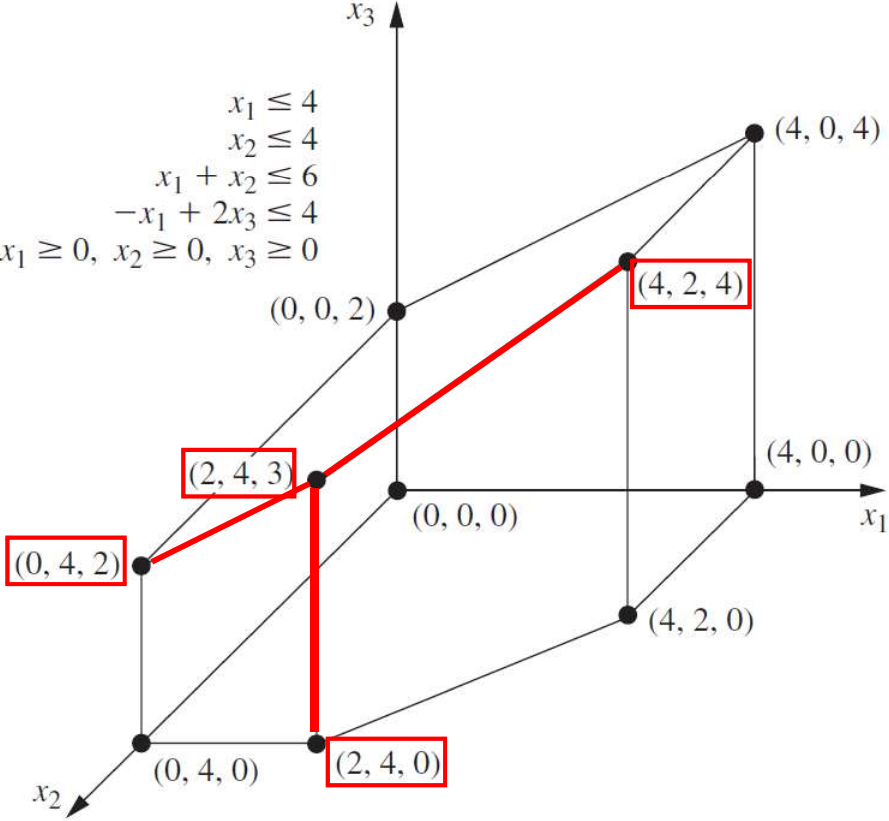
\includegraphics[width = 0.40\linewidth]{Images/43.png}
    \end{center}
    \item \textbf{Molti-a-molti}: I thread a livello utente di un certo processo sono implementati su un insieme di thread a livello del kernel, possibilmente inferiore di numero, e \textbf{l'associazione thread utente/thread kernel è dinamica}, stabilita da uno scheduler interno alla libreria di threading
    \begin{itemize}
        \item Cerca di combinare i vantaggi dei modelli molti-a-uno e  uno-a-uno
        \item \textbf{Svantaggio}: complesso da implementare (la libreria di thread deve dinamicamente alternare l'esecuzione dei thread a livello utente sui thread a livello kernel disponibili)
        \item \textbf{Modello a due livelli}: permette agli utenti di creare dei thread che hanno un mapping uno-a-uno con un thread a livello del kernel
        \item Esempio: Solaris, AIX
    \end{itemize}
    \begin{center}
        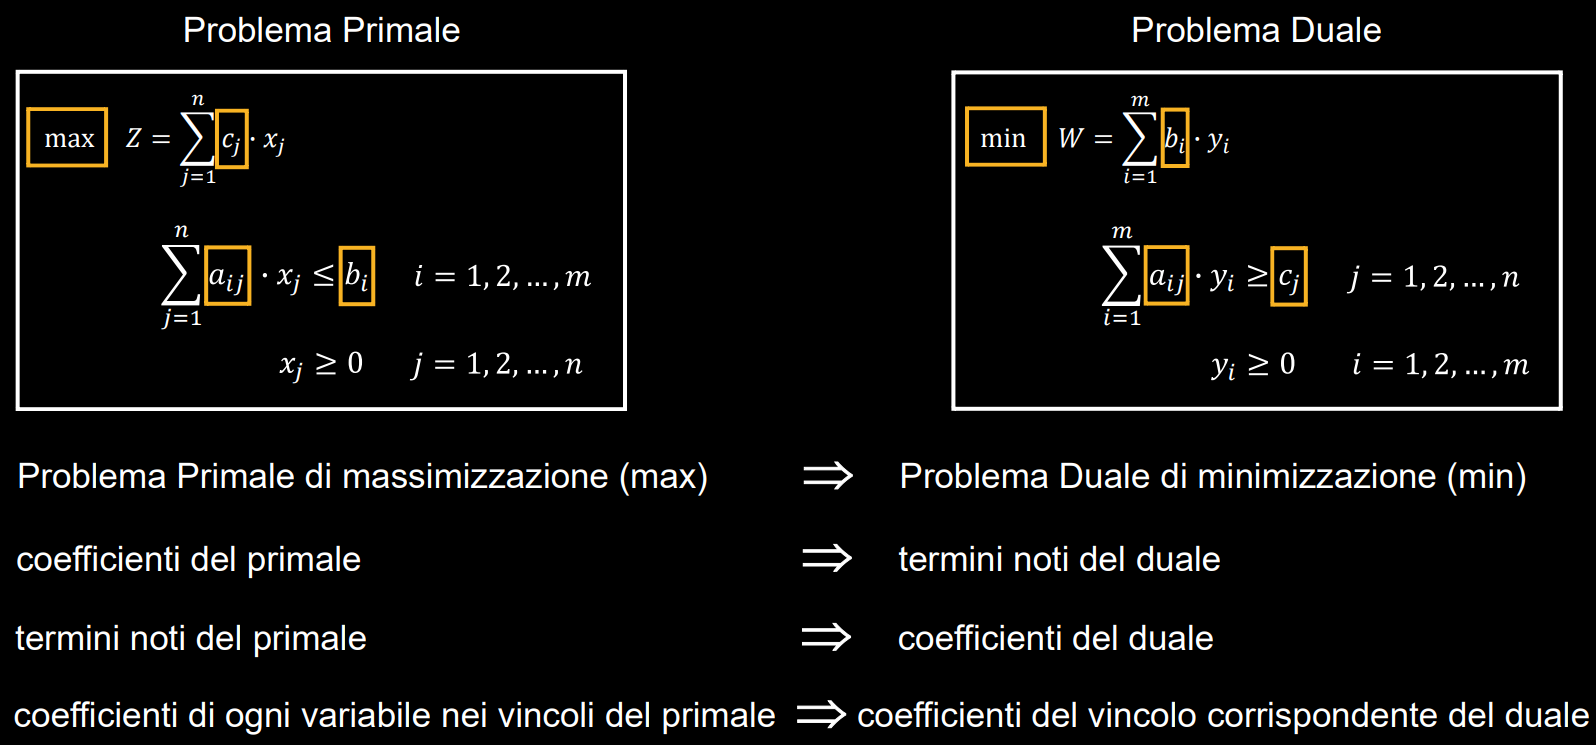
\includegraphics[width = 0.40\linewidth]{Images/44.png}
    \end{center}
\end{itemize}
Nei kernel multithreaded, il kernel mantiene delle strutture dati analoghe ai PCB, i \textbf{thread control blocks} (TCB); un TCB memorizza il
contesto di un thread e le sue informazioni di contabilizzazione.
Il PCB contiene solo le informazioni di contesto e contabilizzazione \textbf{comuni} (ad esempio lo spazio di memoria).
Il PCB è di norma collegato ai TCB dei thread kernel utilizzati dal processo, e viceversa i TCB dei thread kernel utilizzati da un processo sono collegati al PCB del processo.
\subsection{Criteri di valutazione degli algoritmi di scheduling}
In pratica, ogni sistema operativo ha i propri algoritmi di scheduling.
Questo è indizio del fatto che non esiste una politica di scheduling "migliore" di tutte le altre.
\textbf{Necessitiamo quindi di definire delle matriche per confrontare gli algoritmi di scheduling}.
I principali criteri utilizzati sono:
\begin{itemize}
    \item \textbf{Utilizzo della CPU}: percentuale di tempo in cui la CPU è attiva nell'esecuzione dei processi utente (dovrebbe essere tra il 40\% e il 90\%, in funzione del carico)
    \item \textbf{Throughput}: Numero di processi che completano l'esecuzione nell'unità di tempo (dipende dalla durata dei processi)
    \item \textbf{Tempo di completamento}: tempo necessario per completare l'esecuzione di un certo processo (dipende da molti fattori: durata del processo, carico totale, durata dell'I/0...)
    \item \textbf{Tempo di attesa}: tempo trascorso dal processo nella ready queue (meglio del tempo di completamento, meno dipendente dala durata del processo e dall'I/O)
    \item \textbf{Tempo di risposta}: negli ambienti interattivi, tempo trascorso tra l'arrivo di una richiesta al processo e la produzione della prima risposta, sena l'emissione di questa nell'output
\end{itemize}
In questi appunti, terremo in considerazione prevalentemente \textbf{tempo di completamento e di attesa}.
I criteri di valutazione di un algortimo di scheduling sono quindi:
\begin{itemize}
    \item \textbf{Massimo utilizzo della CPU}
    \item \textbf{Massimo Throughput}
    \item \textbf{Minimo tempo di completamento (medio)}
    \item \textbf{Minimo tempo di attesa (medio)}
    \item \textbf{Minimo tempo di risposta (medio)}
\end{itemize}
Naturalmente, nessun algoritmo di scheduling può ottimizzare tutti i criteri contemporaneamente.
\subsection{Principali algoritmi di scheduling}
Presentiamo in questa sezione i principali algoritmi di scheduling.
\subsubsection{Scheduling in ordine di arrivo}
Nello \textbf{scheduling in ordine di arrivo}, o \textbf{first-come-fist-served} (FCFS), la CPU \textbf{viene asseganta al primo processo che la richiede}
\begin{itemize}
    \item \textbf{Vantaggio}: implementazione molto semplice (coda FIFO, nessuna prelazione)
    \item \textbf{Svantaggio}: tempo di attesa medio può essere lungo ("effetto convoglio")
\end{itemize}
\begin{center}
    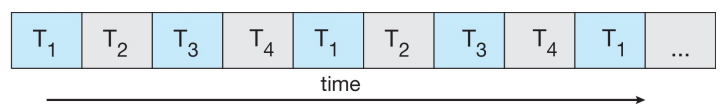
\includegraphics[width = 1\linewidth]{Images/45.png}
\end{center}
\subsubsection{Scheduling per brevità}
Nello \textbf{scheduling per brevità}, o \textbf{shortest-job-first}, la CPU viene assegnata al processo che ha il \textbf{successivo CPU burst più breve}.
\begin{itemize}
    \item \textbf{Vantaggi}: implementazione quasi identica a FCFS, ma \textbf{minimizza il tempo di attesa (è ottimale)}
    \item \textbf{Svantaggio}: di solito non si sa in anticipo qual è il processo che avrà il CPU burst più breve
\end{itemize}
\begin{center}
    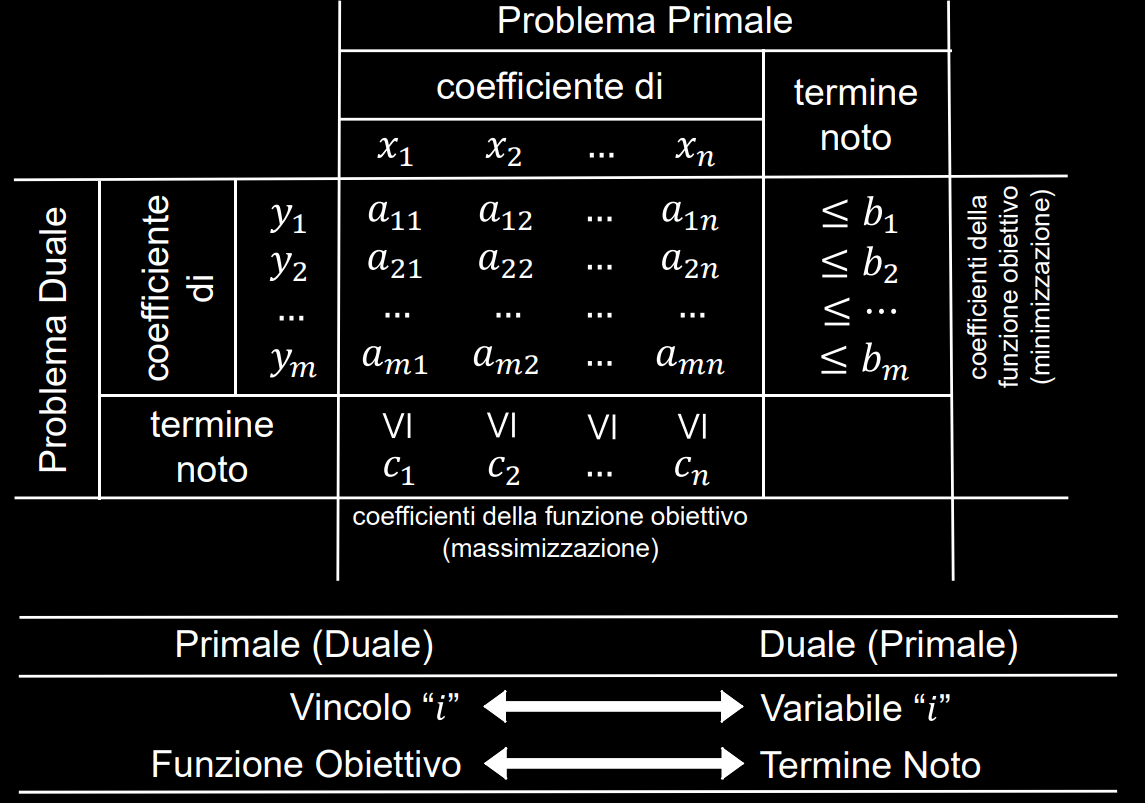
\includegraphics[width = 0.90\linewidth]{Images/46.png}
\end{center}
L'algoritmo \textbf{shortest-remaining-time-first} (SRTF) utiliza la \textbf{prelazione} per gestire il caso in cui i processi non arrivino tutti nello stesso istante:
se nella ready queue arriva un processo con burst più corto di quello running, \textbf{quest'ultimo viene prelazionato dal nuovo processo}. Con preemption e tempo di arrivo:
\begin{itemize}
    \item Il \textbf{tempo di attesa di un processo} è dato da
    $$\textrm{instante di terminazione processo} - \textrm{tempp di arrivo} + \textrm{durata burst}$$
    \item Il \textbf{tempo di completamento} di un processo è invece dato da
    $$\textrm{istante di terminazione processo} - \textrm{tempo di arrivo}$$
\end{itemize}
\subsubsection{Scheduling circolare}
Nello \textbf{scheduling circolare}, o \textbf{round robin (RR)}, ogni processo ottiene una \textbf{piccola quantità fissata di tempo di CPU}, detta \textbf{quanto di tempo}, di solito 10-100 millisecondi, per il quale
può essere in esecuzione. Trascorso tale tempo, il processo in esecuzione viene \textbf{interrotto e messo in fondo alla ready queue}, che è gestita in maniera FIFO.
In tal modo, la ready queue funziona essenzialmente come un \textbf{buffer circolare}, e i processi vengono scanditi dal primo all'ultimo, per poi ripartire dal primo nello stesso ordine.
Per effettuare la prelazione del processo corrente (passaggio del processo da stato running a ready), viene implementato un \textbf{timer} che genera un interrupt periodico con periodo $q$.
Facciamo un esempio con tempo di arrivo $0$ per tutti i processi:
\begin{center}
    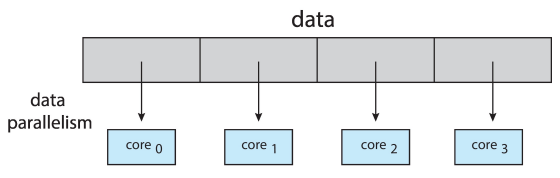
\includegraphics[width = 0.90\linewidth]{Images/47.png}
\end{center}
Lo scheduling circolare presenta le seguenti caratteristiche:
\begin{itemize}
    \item Se ci sono $n$ processi nella ready queue e il quanto temporale è $q$:
    \begin{itemize}
        \item Nessun processo \textbf{attende più di $q(n-1)$} unità di tempo nella ready queue prima di ridiventare running per un altro quanto di tempo (rispetto a SJF e SRTF non c'è bisogno di sapere la durata del burst)
        \item Ogni processo ottiene $1/n$ del tempo totale di CPU, in maniera \textbf{perfettamente equa} (rispetto a SJF e SRTF vengono ottenute solo $q$ unità di tempo per volta)
    \end{itemize}
    \item Comportamento \textbf{in funzione di $q$}:
    \begin{itemize}
        \item $q$ \textbf{elevato}: se $q$ è di regola maggiore della durata di tutti i burst, RR tende al FCFS
        \item $q$ \textbf{basso}: deve comunque \textbf{essere molto più lungo della latenza di dispatch}, altrimenti questa si "mangia" un tempo comparabile al tempo di esecuzione dei processi utente e l'utilizzo della CPU diventa \textbf{inaccetabilmente basso}
    \end{itemize}
    \item \textbf{Performance}:
    \begin{itemize}
        \item Rispetto a SJF, tipicamente RR ha un tempo di completamento medio più alto
        \item Ma \textbf{un tempo di risposta medio più basso} (va bene per i processi interattivi)
        \item Il tempo di completamento medio non necessariamente migliora con l'aumento di $q$
    \end{itemize}
\end{itemize}
\begin{center}
    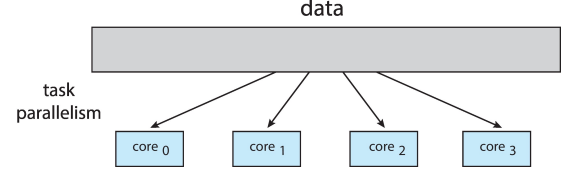
\includegraphics[width = 0.90\linewidth]{Images/48.png}
\end{center}
\subsubsection{Scheduling con priorità}
Nello scheduling con priorità, ad ogni processo è \textbf{associato un numero intero che indica la sua priorità}.
Viene eseguito il processo con più altra priorità, gli altri aspettano (in sistemi UNIX-like, un numero più basso indica una maggiore priorità; in Windows il contrario).
Questo tipo di algoritmi può essere \textbf{preemptive} oppure \textbf{non-preemptive}.
Possono essere permessi più procesi con pari priorità oppure no; in caso positivo occorre stabilire un secondo algoritmo di scheduling per \textbf{abritrare tra i processi a pari priorità} (di solito si utilizza RR).
SJF è un caso particolare di scheduling con priorità, dove quest'ultima l'\textbf{inverso della durata del CPU burst}.
Questi algoritmi soffrono di un problema di \textbf{attesa indefinita} (\textbf{starvation}): un processo a priorità troppo bassa \textbf{potrebbe non venir mai schedulato}.
La \textbf{soluzione} a questo tipo di problema prende il nome di \textbf{invecchiamento} (\textbf{aging}), ossia avviene un \textbf{aumento automatico della priorità di un processo al crescere del tempo di permanenza nella ready queue}.
Facciamo un esempio di scheduling con priorità senza che vi siano processi con la stessa priorità:
\begin{center}
    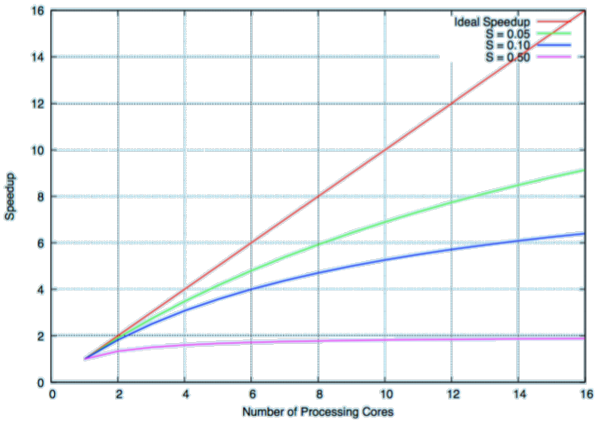
\includegraphics[width = 0.90\linewidth]{Images/49.png}
\end{center}
vediamo invece un esempio con processi con priorità uguali:
\begin{center}
    \includegraphics[width = 0.90\linewidth]{Images/50.png}
\end{center}
\subsubsection{Code multilivello con retroazione}
Lo scheduling con priorità usa \textbf{ready queue separate per ogni priorità}. Viene quindi schedulato il processo nella conda non vuota con priorità maggiore.
\begin{center}
    \includegraphics[width = 0.30\linewidth]{Images/51.png}
\end{center}
Nello scheduling con priorità, in base a quale criterio possiamo assegnare le priorità ai processi?
Un criterio comunemente usato è quello di \textbf{basare la priorità di un processo sul suo tipo}:
\begin{itemize}
    \item \textbf{Priorità più alta ai processi interattivi o cyber-fisici} che devono reagire rapidamente all'I/O (tipicamente I/O bound)
    \item \textbf{Priorità più bassa ai processi che effettuano lunghe computazioni, o processi batch} (tipicamente CPU bound)
\end{itemize}
La priorità di un processo \textbf{può variare dinamicamente}: è sufficiente spostarlo da una ready queue ad una certa priorità all'altra, l'invecchiamento
è di solito implementato in questo modo (spostamento di un processo verso una coda a priorità più alta), ma \textbf{anche l'identificazione di un processo come I/O bound o CPU bound può essere effettuata dinamicamente} e quindi determinare un cambio di priorità, stavolta con uno spostamento verso il basso.
Uno scheduler di questo tipo è detto con \textbf{code multilivello con retroazione}. Questo tipo di schedulero fu introdotto per la prima volta nel sistema operativo CTSS ed è oggi adottato da moltissimi sistemi operativi moderni (Windows, MacOS, FreeBSD, Solaris).
Facciamo un esempio, supponiamo di avere le seguenti code:
\begin{itemize}
    \item $Q_0$: RR con $q_0 = 8$ msec
    \item $Q_1$: RR con $q_1 = 16$ msec
    \item $Q_2$: RR con $q_2 = \infty$ (ossia FCFS)
\end{itemize}
$Q_0$ ha priorità altra, $Q_1$ intermedia e $Q_2$ bassa.
\begin{itemize}
    \item Alla creazione, un processo entra in $Q_0$
    \item Se quando un processo diventa running non termina il suo burst entro il suo quanto di tempo, \textbf{avviene preemption} e viene messo all'inizio della coda \textbf{immediatamente più bassa}, altrimenti rimane nella sua coda.
    \item Per evitare il problema della starvation, \textbf{l'invecchiamento sposta i processi in direzione opposta}, verso le code più alte, se passano troppo tempo in una coda senza essere eseguiti
    \item \textbf{Effetto ricercato}: mantenere i processi I/O bound (con burst della CPU più corti) nelle code a più altra priorità e quelli CPU bound (con burst della CPU lunghi) nelle code a bassa priorità
\end{itemize}
\begin{center}
    \includegraphics[width = 0.50\linewidth]{Images/52.png}
\end{center}
\section{Gestione della memoria: la struttura}
Le arre di memoria che i processori possono usare direttamente per l'esecuzione dei programmi sono solo \textbf{la memoria centrale ed i registri}.
Pertanto, un programma deve essere portato dal disco in memoria centrale perche possa essere eseguito, e il programma deve avere anche \textbf{sufficiente memoria centrale per memorizzare i risultati della computazione}.
La memoria centrale "vede" solo un \textbf{flusso di indirizzi} (richieste di lettura o scrittura) proveniente dal bus di sistema, e \textbf{non è consapevole di chi ha generato tale flusso}.
Le operazioni sui registri richiedono \textbf{un ciclo di clock}, viceversa, le operazioni sulla memoria richiedono \textbf{molti cicli di clock}, anche diverse centinaia, causando uno stallo (stall) del processore, durante il quale
un core multithread può eseguire un altro thread hardware.
Per aumentare l'efficienza degli accessi in memoria, vengono utilizzati diversi livelli di memorie cache tra processore e memoria centrale.






\end{document}
